\RequirePackage[l2tabu, orthodox]{nag}
\documentclass[11pt, a4paper, oneside, openright]{report}

\usepackage[left=30mm, right=20mm]{geometry}
\usepackage[nodayofweek]{datetime}
\newdateformat{mydate}{\monthname \ \THEYEAR}

\usepackage{microtype}
\usepackage{fixltx2e}

\usepackage{parskip}
\usepackage[pagestyles]{titlesec}
\usepackage{fancyhdr}

\usepackage[nottoc,notlof,notlot]{tocbibind}
\usepackage[sort,authoryear]{natbib}

\usepackage[pdftex]{graphicx}

\usepackage{flafter}
%\usepackage{float}
\usepackage{floatrow}
\floatsetup[table]{capposition=top}
\usepackage[titletoc,page]{appendix}
\usepackage[tableposition=top,width=.75\textwidth]{caption}
\usepackage{subcaption}

\usepackage{multirow}
\usepackage{booktabs}
\usepackage{array}

\usepackage{amsfonts}
\usepackage{amsmath}
\usepackage{amssymb}
\usepackage{mathtools}

%\usepackage{amsthm}
%\newtheorem{definition}{Definition}[section]

\usepackage{xcolor}
\usepackage{listings}
\usepackage{verbatim}
\usepackage{algorithm}
\usepackage{algorithmicx}
\usepackage[noend]{algpseudocode}

\usepackage{tikz}
\usetikzlibrary{shapes, arrows, calc, decorations.markings}
\usepackage{pgfplots}

\setcounter{secnumdepth}{3}
\setcounter{tocdepth}{3}
%\setlength\parindent{0pt}

\setlength{\marginparwidth}{2cm}
\reversemarginpar

\lstset{
    language=C++, numbers=left, numberstyle=\tiny, stepnumber=1,
    frame=single, breaklines=true, showstringspaces=false, tabsize=4,
    commentstyle=\itshape\color{gray}, basicstyle=\footnotesize\ttfamily\bfseries, morekeywords={def}
}

\usepackage{url}
\usepackage[bookmarks]{hyperref}

\hypersetup{
    colorlinks=false,
    pdfborder={0 0 0},
    pdftitle={Faster Shortest Path Computation for Traffic Assignment},
    pdfauthor={Boshen Chen}
}

\usepackage[disable, shadow, color=gray!15, linecolor=black]{todonotes} % disable, draft
\newcommand\todoin[2][]{\todo[inline, caption={2do}, #1]{ \begin{minipage}{\textwidth-4pt}#2\end{minipage}}}

\titleformat{\chapter}[display]   
{\normalfont\Huge\bfseries}{\chaptertitlename\ \thechapter}{20pt}{\Huge}   
\titlespacing*{\chapter}{0pt}{-20pt}{1.5em}

\linespread{1.2}

\begin{document}

\pagestyle{fancy}
\fancyhf{ }
\setlength{\headheight}{15.2pt}
\fancyhead[L]{\nouppercase{\leftmark}}
\cfoot[R]{\thepage}

\thispagestyle{empty}
\setcounter{page}{0}
\pagenumbering{Alph}
\begin{titlepage}
    \newcommand{\HRule}{\rule{\linewidth}{0.5mm}}
    \centering
    
\includegraphics[width=0.5\textwidth]{img/logo.jpg}\\[2cm]    
    %\textsc{\LARGE University of Auckland}\\[1.5cm]
    \textsc{\Large Engineering Science}\\[2cm]
    \HRule \\[0.4cm]
    { \huge \bfseries Faster Shortest Path Computation for Traffic Assignment
    }\\[0.4cm]
    \HRule \\[2cm]

    \begin{minipage}{0.4\textwidth}
        \begin{flushleft} \large
            \emph{Author:}\\
            Boshen \textsc{Chen}
        \end{flushleft}
    \end{minipage}
    \begin{minipage}{0.4\textwidth}
        \begin{flushright} \large
            \emph{Supervisors:} \\
            Dr. Andrea \textsc{Raith} \\
            Olga \textsc{Perederieieva}
        \end{flushright}
    \end{minipage}\\[4cm]

    \vfill
    {\large \today}
    \thispagestyle{empty}
\end{titlepage} 

\pagenumbering{roman}

\newpage
\thispagestyle{empty}
\chapter*{Abstract}
The Traffic Assignment (TA) problem involves the selection of optimal path for every vehicle in a transportation network subject to congestion.
One method for solving TA is the Path Equilibration (PE) algorithm.
PE requires to find the shortest path repeatedly between every origin and destination pair in the network for a large number of iterations,
while the travel times of the roads change due to congestion.
The aim of this project is to find a faster shortest path algorithm for PE.
Dijkstra's algorithm, A* search and their bidirectional versions and eight different versions of priority queue data structures that improve these algorithms' performance are implemented.
Two strategies for skipping shortest paths altogether in the iterative environment of PE are also developed.
The first strategy is to avoid the next few iterations when the shortest path of the previous two iterations are the same.
The second strategy is to randomly skip the next shortest path calculation in the hope for the situation where the previous and current iteration is going to be the same.
We present experimental results that demonstrate the run time differences between the priority queues, shortest path algorithms and path calculation skipping strategies.
We conclude A* search algorithm using the priority queue implementation from the C++ standard template library with random skipping strategy has the best performance.

\thispagestyle{empty}
\begin{center}
\Huge Acknowledgements
\end{center}
I would like to thank my superviosrs, Dr Andrea Raith and Olga Perederieieva from the Department of Engineering Science at the University of Auckland,
for their patient guidance, assistance and useful critiques throughout this project.

I would also like to thank my fellow part IV students, especially Danny Tsai and Corey Kok, for their insightful ideas and kind helps, some of the algorithms would take much longer time to write without them.

Finally I would like to thank open-source software,
with out it bidirectional A* search would not have been written.



\setcounter{page}{3}

\renewcommand\contentsname{Table of Contents}
\tableofcontents 
\listoffigures
\listoftables
\listofalgorithms

\newpage
\pagenumbering{arabic}
\setcounter{page}{1}
\chapter{Introduction}
\section{Introduction to traffic modelling}
Nowadays a large portion of people's daily lives involve activities that relate to transportation.
For example, most people need to travel between their workplace and residence twice a day,
or buy goods from shops that need to be delivered across the city.
In the meanwhile, 
transportation networks expand and improve constantly to cater for people's demand for efficient travelling.
but the rate of improvement does not confront with the rate of population growth.
As a result,
the network becomes inefficient, resulting in traffic congestion.

Congestion leads to major economical losses due to time delays and increased usage of petrol.
Congestion causes air pollution that increases respiratory problems such as asthma, 
and the exhaust gas exacerbates global warming.
Congestion also increases noise pollution and causes frustration,
which in turn accelerates traffic accidents.
It is important for traffic designers to be able to reduce congestion problems,
and eliminate its negative effects.
%The transportation network can be improved by, for example,
%introducing road tolls to diverge traffic to less congested roads,
%or by educating people to use public transport.

Making improvements to the transportation network tends to be very costly,
so a good plan is necessary:
use the least amount of investment for the greatest change.
In order to make better plans for traffic design,
different mathematical models have been built to estimate the current and future behaviour of the transportation system.
One particular model called the transportation forecasting model is commonly used.
The aim of this model is to estimate future traffic usage when the system is changed.
For example, changes to a transport system can include upgrading or adding roads, changing roundabouts to traffic lights, or providing better public transport. 

The transportation forecasting model has 4 stages (shown in Figure~\ref{fig:model}):
trip generation, trip distribution, mode choice and traffic assignment \citep{Sheffi}.
In the model, the solution of each stage can be passed to the previous ones to improve transportation forecasting and traffic design.
This means the model can be calibrated numerous times to establish an accurate model which can estimate future traffic behaviour.
In summary, 
the model collects traffic demand data and 
generates origins and destinations for travellers (trip generation).
It then calculates the number of trips that are required between each origin and destination (trip distribution),
and decides which transportation method should be used for each trip (mode choice).
Finally it decides the route (e.g.\ the shortest path) that each trip needs to travel on (traffic assignment), 
where traffic flow is estimated for every modelled road in the network.
The traffic assignment problem in the last stage of the forecast model is a complicated problem.
This is because congestion occurs as traffic flows are assigned onto the network,
and it is very difficult to find an equilibrium situation where everybody in the network finds their best route.
Generally the equilibrium situation happens when it is assumed that people are selfish,
everyone tries to minimise travel times by travelling along their shortest paths.

\begin{figure}[!ht]
    \centering
    \tikzstyle{block} = [rectangle, draw, text width=10em, text centered, rounded corners, minimum height=2em]
    \tikzstyle{line} = [draw, -latex']
    \begin{tikzpicture}[node distance=4em]
        \node [block] (first) {Trip Generation};
        \node [block, below of=first] (second) {Trip Distribution};
        \node [block, below of=second] (third) {Mode Choice};
        \node [block, below of=third] (fourth) {Traffic Assignment};
        \path [line] (second) -- (third);
        \path [line] (first) -- (second);
        \path [line] (third) -- (fourth);
        \path [line] (fourth.west) -- ($(fourth.west)-(0.8,0)$) -- ($(first.west)-(0.8,0)$) -- (first.west);
        \path [line] ($(second.west)-(0.8,0)$) -- (second.west);
        \path [line] ($(third.west)-(0.8,0)$) -- (third.west);
    \end{tikzpicture}
    \caption{Transportation forecasting model}
    \label{fig:model}
\end{figure}

\section{Purpose of this project}
The transportation forecasting model has been implemented in many software packages for traffic design.
One key observation is that,
the traffic assignment problem can take hours, or even days to solve.
It turns out that,
the bottleneck is in the algorithm for solving the shortest path problem.
This is because algorithms for solving the traffic assignment problem are usually iterative,
where each iteration requires to find millions of shortest paths between every origin and destination in the network.
Although each shortest path calculation may take only a fraction of a second,
cumulatively the computational time can be very long.
Therefore the purpose of this project is to find a faster algorithm for solving the shortest path problem in an iterative environment.
As a result, traffic assignment will be solved faster
for larger and more complicated road networks.
This will also allow city designers to estimate traffic flows further into the future and make better decisions on road network design.

In summary,
The algorithms that are going to be studied are:
\begin{itemize}
    \item Bellman-Ford's label correcting algorithm,
    \item Dijkstra's label setting algorithm (using different data structures),
    \item Bidirectional Dijkstra's algorithm,
    \item A* search,
    \item Bidirectional A* search.
\end{itemize}

We also aim to find and discuss the following techniques that can speed up shortest path calculations in an iterative environment:
\begin{itemize}
    \item preprocessing algorithms,
    \item use information from the previous iterations,
    \item avoid shortest path calculations.
\end{itemize}

\section{Structure of the report}
Chapter~\ref{chap:ta} gives a short description of the traffic assignment problem
and presents a specific algorithm called the path equilibration algorithm that solves it.
This algorithm is the begin of our experiments for this project.
Chapter~\ref{chap:solvingspp} introduces the shortest path problem and presents some of the well established algorithms that solve it.
Implementation details are presented in Chapter~\ref{chap:implementation}.
%Strategies for solving the shortest path problem faster in an iterative environment are also described in this chapter.
Chapter~\ref{chap:results} shows the results and discussions for the algorithms described in Chapter~\ref{chap:solvingspp}.
Chapter~\ref{chap:iterative} presents strategies and results for solving the shortest path problem in path equilibration algorithm of the traffic assignment.
Finally conclusions and future work are drawn in Chapter~\ref{chap:conclusions}.


\newpage
\chapter{The Traffic Assignment Problem} \label{chap:ta}

In a transportation network,
every traveller wishes to travel between different pairs of origins and destinations.
As travellers start to travel in the network,
congestion happens and travel speeds tend to decrease rapidly due to more and more interactions between the travellers and the increase in traffic volume.
This leads to the problem of travellers wishing to find the fastest route to travel on,
meanwhile taking account of congestion while every other traveller is trying to do the same.
In transportation modelling point of view,
we wish to find a traffic flow pattern in the network with a given travel demand between the origin and destination pairs. 
This is called the \emph{traffic assignment problem}.

The traffic assignment problem is commonly solved by traffic equilibrium models.
The notion of traffic equilibrium was first formalized by \cite{Wardrop},
where he introduced the postulate of the minimisation of the total travel costs.
His first principle states that ``the journey times on all routes actually used are equal and less than those which would be experienced by a simple vehicle of any unused route.''
%Under the assumption that the travellers have complete knowledge about the network and they always choose the best route to travel based on the current information about the network,
%The principle means that the traffic is in equilibrium when no traveller in the network can find a faster route than the one that is already being travelled on.
The traffic flows that satisfy this principle are referred to as ``user optimal'' flows,
as each traveller chooses the route that is the best for them.
%On the other hand,
%we can also find traffic flows that are ``system optimal'',
%which is characterized by Wardrop's second principle, stating that ``the average journey time is minimum''.

In this chapter,
the network equilibrium model is first stated.
Then a particular solution algorithm for solving such a model is described.
Finally the motivation of this project in the context of solving the traffic assignment problem is brief explained.

\section{The deterministic network equilibrium model}
%In this section,
%the deterministic symmetric network equilibrium model for solving the user optimal of the traffic assignment is summarised.
In order to formulate a mathematical model for solving the traffic assignment problem,
two assumptions are commonly made.
We assume deterministic traffic flows and fixed demand,
and the change of travel time on any link does not depend on the change of traffic flows on the other links.
%These assumptions are commonly made, they allow us to formulate the traffic assignment model as a mathematical program.
%The model assumes the link cost functions are separable, i.e.\ the function values are only dependent on the flows on the link itself, not other flows that do not belong to that link.
%The model also assumes the traffic demand of the network is fixed.

Using notations from \citet{Florian, Florian2008},
we consider a transportation network represented as a graph $G = (N, A)$,
where $N$ is a set of nodes and $A$ a set of directed links in the network.
The number of vehicles (or flow) on link $a$ is $v_a$ ($a \in A)$,
and the cost of travelling on a link is given by the link cost function $c_a(v)$ ($a \in A$),
where $v$ is the vector of link flows over the entire network.

Let $I$ be the set of origin-destination (O-D) pairs
and $K_i$ be the set of cycle-free paths for O-D pair $\forall i \in I$.
The origin to destination traffic demands $g_i$ ($i \in I$) are distributed over directed paths $k \in K_i$,
and it is assumed $K_i \neq \emptyset$ and $K = \cup_{i \in I} K_i$.
Let $h_k$ be the flows on paths $k$ that satisfy the conservation of flow and non-negativity constraints:
\begin{align} \label{eq:ta1}
    \sum_{k \in K_i} h_k & = g_i \quad \forall i \in I, \\
    h_k &\geq 0 \quad \forall k \in K.
\end{align}
The corresponding link flows $v_a$ are given by:
\begin{equation}
    v_a = \sum_{k \in K} \delta_{ak} h_k \quad \forall a \in A,
\end{equation}
where
\begin{equation} \label{eq:ta4}
    \delta_{ak} = 
    \begin{cases}
        1 & \text{if link $a$ is on path $k$},\\
        0 & \text{otherwise}.
    \end{cases}
\end{equation}

In order to solve for user-optimal flows,
the \citet{Wardrop} user-equilibrium condition is applied:
\begin{equation} \label{wardrop1}
    c_k(v^{\ast}) - u_i^{\ast} 
    \begin{cases}
        =0 & \text{if } h_k^{\ast} > 0 \\
        \geq 0 & \text{if } h_k^{\ast} = 0
    \end{cases}
    \quad \forall k \in K_i, i \in I,
\end{equation}
where 
\begin{equation}
    c_k(v) = \sum_{a \in A} \delta_{ak} c_a(v) \quad \forall k \in K,
\end{equation}
and
\begin{equation} \label{wardrop3}
    u_i = \min_{k \in K_i} \left[ c_k(v) \right] \quad \forall i \in I.
\end{equation}

To elaborate, this condition means that the traffic is in equilibrium when no traveller in the network can find a faster route than the one that is already being travelled on.
Furthermore, this condition assumes that the travellers have complete knowledge about the network,
they always choose the best route to travel based on the current information about the network.
This means the equilibrium is the result of everybody simultaneously attempting to minimise their own travel costs.

With constraints \eqref{eq:ta1} - \eqref{eq:ta4},
the user optimal optimisation problem has objective
\begin{equation} \label{eq:user_optimal}
    \min S(v) = \sum_{a\in A} \int_0^{v_a} c_a(x) \mathrm{d} x.
\end{equation}
It has been shown in \citet{Florian} that optimisation problem~\eqref{eq:user_optimal}, \eqref{eq:ta1}-\eqref{eq:ta4} has the user-equilibrium solution as the optimal solution.

The \citet{BPR} (BPR) link cost function
$c_a(v_a)$ is often used to model the travel time on link $a \in A$.
The function is given by
\begin{equation}
    c_a(v_a) = c_f \left(1 + B \left( \frac{v_a}{C_a} \right)^\alpha \right),
\end{equation}
where $B$ and $\alpha$ are the parameters for the level of congestion that can be experienced,
and $c_f$ and $C_a$ are the free-flow travel time and link capacity.
It is important to note this cost function only depends on traffic flow on its own link, and it is strictly monotonic, continuous and differentiable.
An example of this link cost function is shown in Figure~\ref{fig:flowfunction}

\begin{figure}[!ht]
    \centering
    \begin{tikzpicture}
        \begin{axis}
            [
                domain=0:10000,
                black, no markers, smooth,
                xmin=0,xmax=10000,
                ymin=0,ymax=130,
                axis x line=bottom,
                axis y line=left,
                xlabel={Traffic Flow},
                ylabel={Travel Time},
                every axis y label/.style={at={(current axis.above origin)},anchor=north east, xshift=-2pt},
                every axis x label/.style={at={(current axis.right of origin)},anchor=north west, xshift=-2pt},
                extra y ticks={20},
                extra y tick labels={Freeflow time $(c_f)$},
                extra y tick style={overlay},
                xtick=\empty,
                ytick=\empty,
                xticklabel=\empty,
                yticklabel=\empty,
                scaled ticks=false,
                extra x ticks={9000},
                extra x tick style={xticklabel pos=right, xticklabels={Capacity $(C_a)$}, xmajorgrids=true}
            ]
            \addplot [->, black] {20+0.15*(x/2000)^4}; 
        \end{axis}
    \end{tikzpicture}
    \caption{Travel time function.}
    \label{fig:flowfunction}
\end{figure}

\section{Solving the traffic assignment problem}
Different methods exist for solving the traffic assignment problem.
They are classified by how the solution is presented.
They include link-based, path-based and origin-based.
The solution variables for link-based are link flows,
path-based are path flows,
and origin-based are link flows coming from a particular origin.
Summaries of these methods can be found in ~\citet{Zhou2010}.
These solution methods, which have been widely studied,
result different numerical accuracies and vary greatly in run time and memory requirement \citep{Olga2013}.

The deterministic network equilibrium model described in the previous section is equivalent to a convex cost differentiable optimisation problem,
where a wide range of algorithms exists for solving such problem.
They include, the linear approximation method,
the linear approximation with parallel tangents method,
the restricted simplicial decomposition method,
and the path equilibration algorithm \citep{Florian}.

In this project, we focus on the path-based algorithm (also known as path equilibration algorithm) proposed in~\citet{Dafermos1969}.
The algorithm has traditionally been discarded by transportation researchers as too memory-intensive and slow for large networks \citep{Jayakrishnan1994}.
As a result, the development of path-based algorithm has only began in the last decade, and there exist lots of areas for improvement \citep{Olga2013}.

\section{The path equilibration algorithm}
The general approach of the path equilibration algorithm is equivalent to
Gauss-Seidel decomposition, which is an iterative method for solving a linear system of equations.
In a step of the algorithm,
path flows $h_k$ ($\forall k \in K_i$) between a single O-D pair $i \in I$ are considered by keeping the flows of all other O-D pairs fixed.
The algorithm iteratively solves each O-D pair sub-problem until any of them cannot be improved.

The sub-problem for solving each O-D pair $i \in I$ is another fixed-demand network equilibrium problem:
\begin{align} \label{eq:sb1}
    \min & \quad \sum_{a \in A} \int_0^{v_a^i + \bar{v}_a} c_a(x) \mathrm{d} x.\\
    \text{s.t.} &\quad \sum_{k \in K_i} h_k = \bar{g}_i, \quad i \in I, \\
    & \quad h_k \geq 0, \quad k \in K_i,
\end{align}
where flows $\bar{v}_a$ are fixed:
\begin{equation}
    \bar{v}_a = \sum_{i' \neq i} \sum_{k \in K_i} \delta_{ak} h_k,
\end{equation}
and flows $v_a^i$ are varied:
\begin{equation} \label{eq:sb5}
    v_a^i = \sum_{k \in K_i} \delta_{ak} h_k.
\end{equation}

The Gauss-Seidel decomposition (or `cyclic decomposition' by O-D pair) is stated as follows.
\begin{table}[H]
    \begin{tabular}{ m{0.8\textwidth} }
        \hspace{-.5cm}\emph{`cyclic decomposition' by O-D pair} \citep{Florian} \\
        \emph{Step 0.} Given initial solution, set $l = 0$, $l' = 0$.\\
        \emph{Step 1.} If $l' = |I|$, stop; otherwise set $l = l \text{ mod } |I| + 1$ and continue.\\
        \emph{Step 2.} If the current solution is optimal for the $l^\text{th}$ sub-problem \eqref{eq:sb1}-\eqref{eq:sb5}, set $l' = l' + 1$ and return to step 1; otherwise solve the $l^\text{th}$ sub-problem, update the path flows, set $l' = 0$ and return to step 1.\\
    \end{tabular}
\end{table}

The path equilibration algorithm for solving the sub-problem \eqref{eq:sb1}-\eqref{eq:sb5} 
finds the solution of the traffic assignment problem by balancing path flows between each O-D pair,
it finds the shortest and longest path and equalizes the travel times between them.
Let $K_i^{+} = \left\{ k \in K_i | h_k > 0 \right\}$ be the set of paths with positive flows.

The algorithm for solving the $l^\text{th}$ sub-problem of each O-D pair $i \in I$ is stated as follows.
\begin{table}[H]
    \begin{tabular}{ m{0.8\textwidth} }
        \hspace{-.5cm}\emph{Path Equilibration Algorithm} \citep{Florian} \\
        \emph{Step 0}. All-or-nothing assignment: find an initial solution $v_a^i$ and $\bar{v}_a$; $c_a = c_a(v_a^i+\bar{v}_a)$ and the initial $K_i^+$.\\
        \emph{Step 1}. Compute the costs of the currently used paths $c_k$, $k \in K_i^+$. Find $k_1$ such that $c_{k_1} = \displaystyle \min_{k \in K_i} \left[ c_k \right]$ and $k_2$ such that $c_{k_2} = \displaystyle \max_{k \in K_i^+} \left[c_k \right]$.\\
        If $(c_{k_2} - c_{k_1}) \leq \varepsilon$, go to next O-D pair.\\
        \emph{Step 2}. 
        Compute the shortest path $\tilde{k}$ with cost $\tilde{s}_k = \displaystyle \min_{k \in K_i} \left[ c_k \right]$;
        If $\tilde{s}_k < \displaystyle \min_{k \in K_i^+} \left[ c_k \right]$, then the path $\tilde{k}$ is added to the set of kept paths, $K_i^+ = K_i^+ \cup \tilde{k}$.\\
        \emph{Step 3}.  Define the direction $d_{k_1} = (c_{k_2} - c_{k_1})$ for path flow $k_1$ and $d_{k_2} = (c_{k_1} - c_{k_2})$ for path flow $k_2$.
         Find the step size $\lambda$ which redistributes the flow $h_{h_1} + h_{k_2}$ between the paths $k_1$ and $k_2$ using the defined directions $d_{k_1}$ and $d_{k_2}$ in such a way that their costs become equal. That is, shift flow from the longest path to the shortest path in the set of kept path $K_i^+$. \\
        \emph{Step 4}. Using the $\lambda$ obtained, update $h_k = h_k + \lambda d_k, k = \left\{ k_1, k_2 \right\}; v_a^i = v_a^i + \lambda y_a; c_a = c_a(v_a^i + \bar{v}_a)$. \\
    \end{tabular}
\end{table}

In step 0, a so called all-or-nothing assignment is performed for each of the O-D pairs,
where it finds the shortest path for O-D pair $i$ and assigns all traffic supplies along that path to the destination.
In step 1, the two paths that have the minimum and maximum costs are found.
If costs of the two paths are the same, then we can go to the next O-D pair because all travellers have minimised their travel times.
In step 2, since travel times have not been minimised, we improve the currently used paths set from step 1 by computing a new shortest path.
In steps 3 and 4, traffic flows are redistributed between the longest and shortest paths, these steps are equivalent to solving the Wardrop equilibrium shown in Equations~\eqref{wardrop1}-\eqref{wardrop3}.

Keep in mind the all-or-nothing assignment is different from the traffic assignment solution.
The all-or-nothing assignment gives the solution where between every O-D pair,
all traffic flows are assigned along the shortest path.
Meanwhile the traffic assignment gives the solution where every individual traveller travels along their shortest path,
so between O-D pairs, there is a set of paths with different traffic flows.
This is presented by the set of kept path $K_i^+$ in the path equilibration algorithm.

In summary, in each iteration of the path equilibration algorithm,
it first computes the shortest path with fixed traffic flows and link costs for O-D pair $i \in I$, moves the traffic flow closer to satisfying the Wardrop equilibrium,
updates all the link costs and finally continues with the next O-D pair.

Path equilibration is said to be memory intensive because for each O-D pair, it has to store all of the kept path $K_i^+$.
On networks with millions of O-D pairs, the algorithm may require more than 10 gigabytes of memory, as our algorithms show.

If we are given a large network and assume it requires many iterations to find the optimal solution,
it can be shown that a large number of shortest path calculations are needed.
For example, 
given the algorithm takes 20 iterations to solve a small network with $100,000$ O-D pairs,
it require more than 6 minutes to solve if
each shortest path calculation consumes 0.01 second.
In reality,
networks may contain millions of O-D pairs.
Thus for this project we wish to
investigate and find a faster shortest path algorithm,
and also investigate other ways of improving solution time for the traffic assignment problem.

\section{Convergence and stopping criterion} \label{sec:convergence}
For completeness, the convergence criterion for the traffic assignment is discussed in this section.
It it known that the objective function~\eqref{eq:user_optimal} of the problem is convex (any local minimum is also the global minimum),
so the convergence of the Gauss-Seidel strategy is ensured \citep{Florian2008}.
The convergence criterion of traffic assignment algorithms is normally measured by so called relative gap \citep{Rose}.
\cite{Rose} states that ``the relative gap is expressed by the difference between the current value of 
the objective function and the lower bound as a percentage of the current objective function.''
Here the objective function is the user equilibrium (UE) solution of the traffic assignment problem.
And the lower bound refers to the all-or-nothing (AON) assignment in step 0 of the path equilibrium algorithm.

The relative gap (RGAP) is computed as
\begin{equation}
    \text{RGAP} = \frac{\text{UE} - \text{AON}}{\text{UE}} = \frac{\sum_{a \in A} v_a c_a - \sum_{i \in I} g_i c_{\tilde{k}_i}}{\sum_{a \in A} v_a c_a}.
\end{equation}
The AON solution is the sum of travel times $c_{\tilde{k}_i}$ of each traffic demand $g_i$ travelling on their shortest path $\tilde{k}_i$.
The UE solution is the sum of travel times over the entire network.
These two values are improved from iteration to iteration during the path equilibration algorithm until they become identical, i.e.\ RGAP converges to 0.
The traffic assignment problem is solved when RGAP is 0,
but normally we stop the algorithm at some tolerance such as $10^{-6}$.

It is worth to note that the speed of convergence is highly dependent on how small the relative gap is set,
as well as the size and complexity of the network.
A smaller relative gap will result in more iterations for the traffic assignment algorithms.


\newpage
\chapter{Solving the shortest path problem}
\label{chap:solvingspp}

Over the years,
various algorithms have been developed 
to address the problem of finding the shortest path.
This chapter states notations and definitions for the shortest path problem and discusses
the theory of solving it.
Algorithms that are applicable for the traffic assignment problem are summarised,
including the discussion of their advantages and drawbacks.

\section{Notations and definitions}
The Shortest Path Problem (SPP) is the problem of finding the shortest path from a given origin  to some destination.
There are two types of SPP that are going to
be analysed in this chapter:
a single-source and a point-to-point SPP.  
More emphasise is going to be put on the point-point-point SPP for the path equilibration algorithm described in the previous chapter.
%The Frank-Wolfe algorithm in the TA involves
%solving the single-source SPP by finding shortest path going from one origin to every other destinations of the network.
%The Path Equilibration method in the TA
%Solving the point to point SPP solves from one origin to a specific destination and is used in the Path Equilibration method. 

%When solving SPP for a normal road network,
%different measurements such as distance and travel exist for the road length.
%But in traffic assignment,
%the road length is measured in a non-decreasing travel time function,
%which encapsulates information such as traffic flow, road capacity and travel speed.
%This travel time function (Figure~\ref{fig:flowfunction}) is always non-negative so taking advantage of this helps the selection of algorithms that uses this property.

Now we present the notations mainly borrowed from \citet{Cormen} and \citet{Klunder}.
We denote $ G = ( N, A ) $ a weighted, directed graph,
where $ N $ is the set of nodes (origins, destinations, and intersections)
and $ A $ the set of arcs (roads).
We say $ A $ is a subset of the set $ \{ (u, v)\, | \, u, v \in N \} $ of all ordered pairs of nodes.
We denote the link cost function $ c : A \rightarrow \mathbb{R} $ which assigns a cost (travel time) to any arc $ (u,v) \in A $ depending on traffic flow on that arc.
We write the costs of arc $(u, v)$ as: $ c((u, v)) = c_{uv} $.

The path $P$ inside a transportation network has to be a directed simple path, 
which is a sequence of nodes and edges $ (u_1, (u_1, u_2), u_2, \ldots , (u_{k-1}, u_k), u_k ) $
such that $ (u_i, u_{i+1}) \in A$ for $i = 1,\ldots,k-1$ and $u_i \neq u_j$ for all $ 1 \leq i < j \leq k$.
Note $u_1$ is the origin and $u_k$ is the destination of the path $P$, $u_1$ and $u_k$ together is called an O-D pair for this path.
For simplicity, we denote $s$ to be the source (origin) and $t$ to be the target (destination) for any path $P$.
%Finally we denote cost of the whole path $C(P) := \sum_{(u,v)\in P} c_{vw}$.

In traffic assignment,
the origin and destination nodes used for traffic supply and demand are referred as zone nodes.
The zones are conceptual nodes that are untravellable in the network,
which means a path between two zone nodes must pass through another zone node.
Figure~\ref{fig:zonenodes} demonstrates how a zone node behaves under different conditions.
If the zone is an origin node, then only emanating arcs are allowed.
If it is a destination node, then only emerging arcs are allowed.
And if it is neither, then no arcs can pass through it.
\begin{figure}[H]
    \tikzstyle{main node} = [circle, draw, text centered, minimum height=2.5em]
    \tikzstyle{line} = [->, draw]
    \centering
    \begin{subfigure}[b]{0.4\textwidth}
        \centering
        \begin{tikzpicture}[>=stealth', line width=1pt, auto, node distance=3cm]
            \node[main node] (zone) {zone};
            \node[main node] (1) [below left of=zone] {1};
            \node[main node] (2) [below right of=zone] {2};
        %\path [line, red] (1) -- (zone);
            \path [line, green!80!black] (zone) -- (2);
            \path [line, green!80!black] (1) -- (2);
            %\node (text) [yshift=-5em,above of=zone] {origin node};
        %\node at ($(zone) !.5! (2)$) {$\mathbin{\tikz [x=1.4ex,y=1.4ex,line width=.3ex, black] \draw (0,0) -- (1,1) (0,1) -- (1,0);}$};
        \end{tikzpicture}
        \caption{zone as origin node}
    \end{subfigure}
    \quad
    \begin{subfigure}[b]{0.4\textwidth}
        \centering
        \begin{tikzpicture}[>=stealth', line width=1pt, auto, node distance=3cm]
            \node[main node] (zone) {zone};
            \node[main node] (1) [below left of=zone] {1};
            \node[main node] (2) [below right of=zone] {2};
            \path [line, green!80!black] (1) -- (zone);
        %\path [line, red] (zone) -- (2);
            \path [line, green!80!black] (1) -- (2);
            %\node (text) [yshift=-5em,above of=zone] {destination node};
        %\node at ($(zone) !.5! (2)$) {$\mathbin{\tikz [x=1.4ex,y=1.4ex,line width=.3ex, black] \draw (0,0) -- (1,1) (0,1) -- (1,0);}$};
        \end{tikzpicture}
        \caption{Zone as destination node}
    \end{subfigure}

    \vspace{1cm}
    \begin{subfigure}[t]{\textwidth}
        \centering
        \begin{tikzpicture}[>=stealth', line width=1pt, auto, node distance=3cm]
            \node[main node] (zone) {zone};
            \node[main node] (1) [below left of=zone] {1};
            \node[main node] (2) [below right of=zone] {2};
        %\path [line, green!80!black] (1) -- (zone);
        %\path [line, red] (zone) -- (2);
            \path [line, green!80!black] (1) -- (2);
            %\node (text) [yshift=-5em,above of=zone] {neither};
        %\node at ($(zone) !.5! (2)$) {$\mathbin{\tikz [x=1.4ex,y=1.4ex,line width=.3ex, black] \draw (0,0) -- (1,1) (0,1) -- (1,0);}$};
        \end{tikzpicture}
        \caption{Zone as neither origin nor destination node}
    \end{subfigure}
    \caption{Zone node and its allowable arc flows}
    \label{fig:zonenodes}
\end{figure}

\begin{comment}
Through out the report,
run-time analysis (big O and other notations) is used to demonstrate the estimation of algorithm running time regarding their input size. 
\todo[inline]{How do I nicely say `let the reader refer to other resources?'
or do I describe what big O notation is?}
\end{comment}

\section{Generic shortest path algorithm}
A family of algorithms exist for solving the shortest path problem.
In this section the generic case for these algorithms are described.

This family of algorithms aims to find a 
distance label vector ($d_1, d_2,\dots, d_v$),
and the corresponding shortest path between each origin and destination \citep{Klunder}.
Each $d_v$ tracks the least distance of the path going from the origin $s$ to an destination $v$.
We denote $d_v = \infty$ if no path has been found.
A shortest path is optimal when it satisfies the following conditions:
\begin{align}
    d_v \leq d_u + c_{uv}, \quad \forall(u,v) \in A, \label{eq:Bellman1}\\
    d_v  =   d_u + c_{uv}, \quad \forall(u,v) \in P. \label{eq:Bellman2}
\end{align}
The inequalities~(\ref{eq:Bellman1}) are called Bellman's condition \citep{Bellman}.
To solve the shortest path problem,
we wish to find a label vector $d$ which satisfies Bellman's condition for all of the nodes in the graph.
Algorithms for solving the SPP generally uses some kind of queue $\mathcal{Q}$ to store the label distances $d$.

In the label vector,
a node is said to be unvisited when $d_u = \infty$.
Scanned and still in the queue when $d_u \neq \infty$.
Labelled when the node has been retrieved from the queue and its distance label cannot be improved further.
If a node is labelled then its distance value is guaranteed to represent the minimal distance from $s$ to $t$.

In the generic shortest path algorithm,
the algorithm continuously finds the node that violets the Bellman's condition (\ref{eq:Bellman1}) and updates its distance label with the path that have a shorter distance that connects to it.
All shortest paths connecting the origin $s$ to all other nodes in $N$ is found when both Equation~\ref{eq:Bellman1} and \ref{eq:Bellman2} hold.
It is important to note that arcs with negative costs are permitted,
but the graph must not contain negative cycles.
%In the generic shortest path algorithm,
%we start by putting the origin node in the queue,
%and then iteratively find the arc that violates the Bellman's condition (i.e., $d_v > d_u + c_{uv}$).
%Distance labels are set to a value which satisfies condition (\ref{eq:Bellman1}) to the corresponding node of that arc.
%Shortest path going from $s$ to all other nodes in $N$ is found when (\ref{eq:Bellman1}) is satisfied for all edges in $A$.
%It may not be obvious but negative costs are permitted in the GSP but not negative cost cycles.

To keep track of the shortest path found so far for node $u$,
we denote $p_u$ the predecessor of node $u$.
The shortest path can be constructed by following the predecessor of the destination node $t$ back to the origin node $s$.
We set $p_s = -1$ to indicate it does not have a predecessor.

Algorithm~\ref{algo:gsp} \citep{Klunder} describes the generic shortest path algorithm mentioned above,
with an extra constraint required when solving a TA problem: travelling through zone nodes is not permitted.
In essence, this algorithm repeatedly selects node $u\in\mathcal{Q}$ and 
updates its distance label if the Bellman's condition is violated for all its emanating edges.

\begin{algorithm}[H]
    \caption{The Generic Shortest Path Algorithm}
    \label{algo:gsp}
    \begin{algorithmic}[1]
        \Procedure{GenericShortestPath}{$s$}
        \State $\mathcal{Q} \gets \mathcal{Q} \cup \{s\}$ \Comment{initialise queue with source node}
        \State $p_s \gets -1$ \Comment{origin has no predecessor}
        \State $d_s \gets 0$
        \ForAll {$ u \in N : u \neq s $} \Comment{all nodes are unvisited except the source}
        \State $d_u \gets \infty$
    \EndFor

    \While{ $\mathcal{Q} \neq \emptyset$ }
    \State $ u \gets \text{next}(\mathcal{Q}) $ \Comment{select next node}
    \State $ \mathcal{Q} \gets \mathcal{Q} \setminus \{u\} $
    \If{ $u \neq \text{zone} $}
    \ForAll {$v : (u, v) \in A$} \Comment{check Bellman's condition for all successors of $u$}
    \If {$d_u + c_{vw} < d_v$}
    \State $d_v \gets d_u + c_{vw}$
    \State $p_v \gets u$
    \If {$v \notin \mathcal{Q}$} 
    \State $\mathcal{Q} \gets \mathcal{Q} \cup \{v\}$ \Comment{add node $v$ to queue if unvisited}
\EndIf
                    \EndIf
                \EndFor
            \EndIf
        \EndWhile
    \EndProcedure
\end{algorithmic}
\end{algorithm}

Algorithm~\ref{algo:gsp} is generic because of two reasons:
the rule for selecting the next node $u$ (the `next' function in line 8) and
the implementation for the queue $\mathcal{Q}$ is unspecified.
Different algorithms use different rules and implementations to give 
either the one-source or the point-to-point shortest path algorithm \citep{mplomer}.
The rules and implementations are described in the following sections to give concrete algorithms for solving the SPP.

\section{Bellman-Ford-Moore algorithm} \label{section:labelcorrectingalgorithm}
When some specific strategy is applied to maintain the queue $\mathcal{Q}$
and arc costs are allowed to have negative values,
the generic shortest path algorithm is addressed as the label correcting algorithm,
or Bellman-Ford-Moore algorithm (credited to \citet{Bellman, Ford} and \citet{Moore}).

In this algorithm,
the distance labels do not get permanently labelled when the next node in the queue is retrieved.
Another node may `correct' this node's distance label again,
thus the name label correcting algorithm.

One specific strategy for maintaining the queue is described in \citet{Sheffi}.
This strategy is shown to be very effective for computing shortest path on transportation networks.
It avoids duplicating computation by not physically moving nodes in the queue,
as well as not adding nodes to the queue if they are already in it.
The nodes in the queue are simply processed from front to end.
Scanned nodes are firstly added to the end of the queue,
and if the scanned node is already in the queue,
then the node is put in front of the queue so they can processed first.
This strategy transforms the queue into a first-in-first-out (FIFO) queue.

In order to satisfy the Bellman's condition for all edges,
the algorithm has to scan all edges $|N|-1$ times,
resulting a run time of $O(|N||A|)$.

\section{Dijkstra's algorithm} \label{sec:dijkstra}
The classic algorithm for solving the single-source shortest path problem is the label setting algorithm published by \citet{Dijkstra}.
The algorithm is addressed as label setting because when the next node $u$ is retrieved from the queue,
it gets permanently labelled;
the shortest path going to this node is solved and 
the distance label represents the length of its shortest path.
In order to achieve label setting, 
it is assumed that all arc costs are non-negative,
and queue is modified to always have the minimum distance label in the front.
This modification allows the algorithm to visit every node in the graph exactly once,
where the next node is labelled in the order of non-decreasing distance labels.

The advantage of this algorithm is that,
when the next labelled node is the destination node,
the algorithm can be stopped for the point-to-point shortest path problem.
This reduces the total run time as the algorithm does not have to scan the entire graph,
which is desirable for the Path Equilibration algorithm described in the previous chapter.

\subsection{Priority queues} \label{sec:pq}
The run time performance of Dijkstra's algorithm depends heavily on the implementation of the queue for storing the scanned nodes.
\citet{Cormen} suggests the use of min-priority queues.
Min-priority queues are a collection of data structures that always serve the element with highest priority.
In the shortest path problem, the priority is measured by the distance labels, where smaller distance label have higher priority.

Algorithm~\ref{algo:p2pdijkstra} shows the use of the min-priority queue in Dijkstra's algorithm.
The min-priority queue has 3 main operations: Insert, Extract-Min and Decrease-Key.
The Insert operation (line $2$ and $17$) is used for adding new nodes to the queue.
The Extract-Min operation (line 8) is used for getting the element with the minimum distance label.
And the Decrease-Key (line 19) is used for updating the distance label if the node is already in the queue.

\begin{algorithm}[H]
    \caption{Point to Point Dijkstra's Algorithm}
    \label{algo:p2pdijkstra}
    \begin{algorithmic}[1]
        \Procedure{Dijkstra}{$s, t$}
        \State $\text{Insert}(\mathcal{Q}\text{ , u})$ \Comment{initialise priority queue with source node}
        \State $p_s \gets -1$ \Comment{origin has no predecessor}
        \State $d_s \gets 0$
        \ForAll {$ u \in N : u \neq s $} \Comment{all nodes are unvisited except the source}
        \State $d_u \gets \infty$
    \EndFor

    \While{ $\mathcal{Q} \neq \emptyset$ }
    \State $ u \gets \text{Extract-Min}(\mathcal{Q}) $ \Comment{select next node with minimum value}
    \If{ u = t}
    \State $\text{Terminate Procedure}$ \Comment{finish if next node is the destination}
\EndIf
\If{ $u \neq \text{zone} $}
\ForAll {$v : (u, v) \in A$} \Comment{check Bellman's condition for all successors of $u$}
\If {$d_u + c_{vw} < d_v$}
\State $d_v \gets d_u + c_{vw}$
\State $p_v \gets u$
\If {$v \notin \mathcal{Q}$} 
\State $\text{Insert}(\mathcal{Q}, v)$ \Comment{add node $v$ to queue if unvisited}
\Else
\State $\text{Decrease-Key}(\mathcal{Q}, v)$ \Comment{else update value of $v$ in queue}
    \EndIf
\EndIf
                \EndFor
            \EndIf
        \EndWhile
    \EndProcedure
\end{algorithmic}
\end{algorithm}

According to \citet{Cormen},
a min-priority queue can implemented via an array, a binary min-heap or a binary search tree,
where each implementation give different run time performances.

In the array implementation,
the distance labels are stored in an array where the $n^{\text{th}}$ position gives the distance value for node $n$.
Each Insert and Decrease-Key operation in this implementation takes $O(1)$ time, and each Extract-Min takes $O(|N|)$ time (searching through the entire array), giving a overall time of $O(|N|^2 + |A|)$.

A binary min-heap is a binary tree that satisfies the min-heap property:
the value of each node is smaller or equal to the value of its child nodes.
\citet{Cormen} shows that the performance of the Dijkstra's algorithm can be improved with a binary min-heap if the graph is sufficiently sparse (in particular $A = o(|N|^2/\log(|N|))$.
In this implementation, each Insert and Extract-Min operation takes $O(\log(|N|))$ time for each $|N|$,
and the Decrease-Key operation takes $O(\log(|N|))$ time for each $|A|$.
The total running time of Dijkstra's algorithm using min-priority is therefore $O((|N|+|A|)\log(|N|))$,
which is an improvement compared to the array implementation.

The running time can be further improved using a Fibonacci heap developed by \citet{Fredman}.
Historically, the development of the Fibonacci heap was motivated by the observation that Dijkstra's algorithm typically does more Decrease-Key operation compared to the Extract-Min operation.
In Fibonacci heap, each of the $|N|$ Extract-Min operation takes $O(\log(|N|))$ amortized time
and each of the $|A|$ Decrease-Key operation takes only $O(1)$ amortized time.
The total running time is therefore $O(|N| \log(|N|)+|A|)$,
which is a further improvement.

Min-priority queue can also be implemented as a binary search tree.
In a binary search tree, the worst case for insertion, deletion and search for an element all have $O(\log(|N|))$ time.
Dijkstra's algorithm can easily be modified to accommodate a binary search tree:
when label distance of a node need to be updated,
we remove that node from the tree and insert a new one with the updated value (this is analogous to the Decrease-Key operation).
Dijkstra's algorithm using a binary search runs $O((|N|+|A|)\log(|N|))$ in the worst case, which is the same compared to the min-binary heap implementation.
The advantage of using a binary search tree is that we do not have to keep track of information about whether a node is in the queue,
this is because when performing the Decrease-Key operation,
we simply delete the node and add a new node with the updated value.

\section{Bidirectional Dijkstra's algorithm} \label{section:bidirectional}
Dijkstra's algorithm can be imagined to be searching radially outward in a circle with the origin in the centre and destination on the boundary.
Likewise, Dijkstra's algorithm can be used on the reverse graph (all edges reversed in the graph) from the destination node.
Thus Dijkstra's algorithm can be started from the origin and destination at the same time.
The motivation for doing this is because the number of scanned nodes can be reduced when searching bidirectionally:
two smaller circles growing outward radially instead of a larger one.
Figure~\ref{fig:bidirect} demonstrates the difference in search area between a normal Dijkstra's algorithm and its bidirectional version,
it is easy to see that the total search area of the bidirectional version is a lot smaller.

\begin{figure}[H]
    \tikzstyle{main node} = [circle, draw, text centered, minimum height=2.5em]
    \tikzstyle{big circle} = [circle, draw, dashed, text centered, minimum height=8em]
    \tikzstyle{small circle} = [circle, draw, dashed, text centered, minimum height=5em]
    \centering
    \begin{subfigure}[t]{.4\textwidth}
        \centering
        \begin{tikzpicture}[>=stealth', line width=1pt, auto, node distance=2cm]
            \node [main node] (s)  {s};
            \node [main node] (t) [right of=s] {t};

            \node [big circle] at (s) {};
        \end{tikzpicture}
        \caption{Dijkstra's algorithm}
    \end{subfigure}
    \begin{subfigure}[t]{.4\textwidth}
        \centering
        \begin{tikzpicture}[>=stealth', line width=1pt, auto, node distance=2cm]
            \node [main node] (s) {s};
            \node [main node] (t) [right of=s] {t};

            \node [small circle] at (s) {};
            \node [small circle] at (t) {};
            \node [big circle, white] at (s) {};
        \end{tikzpicture}
        \caption{bidirectional}
    \end{subfigure}
    \caption{Difference between the scan area of label setting and its bidirectional version}
    \label{fig:bidirect}
\end{figure}

It is common to conclude that the shortest path is found when the two searches meet somewhere in the middle,
but this is not actually the case.
There may exist another arc connecting the two frontiers of the searches that has a shorter path (see \citet{Klunder} for the proof).
The correct termination criteria was first designed and implementation by \citet{Pohl} based on researches presented by \citet{Dantzig, Nicholson} and \citet{Dreyfus}.
The procedure and algorithm is summarised in \citet{Klunder}, and the termination criteria is presented by \citet{Pohl}.

The bidirectional search algorithm is shown in Algorithm~\ref{algo:bidirectional}.
Two independent Dijkstra's algorithms are alternatively run on the forward and reverse graph (forward and backward algorithm).
The algorithm terminates when some node is permanently labelled in both directions.
Once the algorithm has terminated,
the correct shortest path is found by looking for a arc connecting the frontiers of the two searches that may yield a shorter path.
This extra requirement increases the run time significantly, 
where searches are needed for all edges that connect all labelled nodes in the forward search to all labelled nodes in the backward search.

Note in Algorithm~\ref{algo:bidirectional},
$\mathcal{R}^s$ contains the set of nodes in the forward search that are permanently labelled from the origin node,
which have corresponding label distances $d_v^s$.
Similarly, $\mathcal{R}^t$ contains contains the set of nodes in the backward search that are permanently labelled from the destination node,
which have corresponding label distances $d_v^t$.

\begin{algorithm}[H]
    \caption{Bidirectional Dijkstra's Algorithm}
    \label{algo:bidirectional}
    \begin{algorithmic}[1]
        \Procedure{Bidirectional}{$s, t$}
        \State Execute one iteration of the forward algorithm.
        If the next node $u$ is labelled permanently by the 
        backward algorithm $(u\in\mathcal{R}^t)$, go to step 3.
        Else, go to step 2.
        \State Execute one iteration of the backward algorithm.
        If the next node $u$ is labelled permanently by the
        forward algorithm $(u\in\mathcal{R}^s)$, go to step 3.
        Else, goto step 1.
        \State Find $\min\{\min\{d_v^s + c_{vw} + d_w^t | v \in \mathcal{R}^s, w \in \mathcal{R}^t, (v, w) \in A\}, d_u^s + d_u^t\}$, which gives the correct shortest path between $s$ and $t$.
    \EndProcedure
\end{algorithmic}
\end{algorithm}

In recent years,
\citet{Goldberg05} improved the bidirectional algorithm using a better termination condition,
where step 3 of Algorithm~\ref{algo:bidirectional} is embedded during the searches.
The termination condition is summarized as the following.
During the forward and backward search,
we maintain an extra variable, $\mu$, to present the length of shortest path seen so far during the forward and backward search.
Initially $\mu = \infty$.
When an arc $(v,w)$ is visited by the forward search and the node $w$ has been scanned in the backward search, or vice versa,
we know the shortest path $s-v$ and $w-t$ have lengths $d_v^s$ and $d_w^t$ respectively.
During the search, if $\mu > d_v^s + c_{vw} + d_w^t$ then the current connected path $s-v-w-t$ is shorter than the one before, 
so we update $\mu = d_v^s + c_{vw} + d_w^t$.
The algorithm terminates when a node is permanently labelled in both directions,
where $\mu$ gives the shortest path length.

\citet{GoldbergEPP} showed and proved a stronger termination condition on top of his previous one.
The searches can be stopped if the sum of the two top priority queue values is greater than $\mu$,
\[
    \text{top}_f + \text{top}_r \geq \mu,
\]
where $\text{top}_f$ and $\text{top}_r$ are the next minimum distance labels that have not been labelled in the forward and backward search.

Overall, the bidirectional version of Dijkstra's algorithm is faster than the single direction one if it is implemented correctly using the best termination criterion.

\section{A* Search}\label{section:A*}
Dijkstra's algorithm can be imagined as growing the shortest path tree radially out from the origin,
the location of the destination does not affect how the shortest path tree is grown.
In fact, heuristic estimates can be used to guide the shortest path tree toward the destination,
forming an ellipsoid shape.
The use of heuristic estimates was first described by \citet{Astar},
where the algorithm is given the name A* search.
A* search is a goal directed search where the direction of search is aimed toward the destination.

%In traditional road networks,
%straight Euclidean distances are used for the heuristic estimates.

Formally we define the following.
Let $h_v$ be the heuristic estimate for the shortest path distance between node $v$ to destination $t$.
We apply Bellman's conditions such that an optimal solution exist, that is 
\begin{align}
    &h_v \leq h_u + c_{uv} \quad \forall(u,v) \in A, \label{eq:A*1}\\
    &h(t) = 0. \label{eq:A*2}
\end{align}

Although $h_v$ is a heuristic function,
optimal solution can still be achieved under the following conditions.
\citet{Astar} states that the heuristic estimate function $h$ must be admissible and consistent.
In context of road networks that use geographical coordinates and Euclidean distances,
admissible means that the heuristic must never over-estimate the distance to the goal.
And consistent means that the estimated length of a node reaching its destination must not be greater than the estimated length of its predecessors (i.e.\ Equation~\ref{eq:A*1} and \ref{eq:A*2}).
This two conditions mean that if the heuristic estimate is the shortest path distance from each node to the destination,
and the estimate is smaller than or equal to the actual distance going to that destination,
then the optimal shortest path can always be found. 

%Note a consistent heuristic is also admissible but not the opposite.
%\citet{Astar} proves if the heuristic function (such as using geographical coordinates and Euclidean distance) is admissible and consistent,
%then A* is guaranteed to find the correct shortest path with a better time performance by scanning less nodes and edges.

To implement A* search,
Dijkstra's algorithm is modified.
When a node $v$ is about to be added to the priority queue,
the heuristic estimate $h_v$ is calculated.
Compared to Dijkstra's algorithm,
instead of inserting node $v$ with its distance label $d_v$,
we now insert with $d_v + h_v$.
By doing so,
nodes that are closer to the destination are now labelled first.

In graphs that are measured by Euclidean distances,
the heuristic estimate $h_u$ is the straight Euclidean distance between node $u$ and destination $t$.
But in our traffic assignment problem,
geographical coordinates and Euclidean distances can not be used.
This is because the length of the arcs are determined by the BPR link cost function,
where it determines the travel time on the link based on the traffic flow.
When the traffic assignment is getting solved,
there are only two ways to obtain the travel time estimate from any given node to the destination.
They are either to use the travel time from the previous iteration,
or use the zero-flow travel times.

It is obvious that using travel times from the previous iteration do not work.
This is because traffic flows can decrease between iterations.
The decreased traffic flows result not admissible travel times,
where some of the arc travel times from the previous iteration is now longer than the current travel times.
Using these longer travel times from the previous iteration will overestimate the travel time for the current iteration,
which results the shortest path not being able to be calculated.

Another option is to use zero-flow travel times for the heuristic estimates.
The estimates can be obtained from computing the shortest path tree for every node where the traffic flow of the entire network set to 0.
So for any O-D pair, the corresponding $h_u$ is equivalent to the travel time of the shortest path from node $u$ to its destination.
These computed zero-flow travel times are both admissible and consistent.
This can be shown by analysing the BPR link cost function shown in Figure~\ref{fig:flowfunction}.
The function is a monotonic non-decreasing function with the lowest value being the zero-flow travel times.
As traffic flows change from iteration to iteration,
the travel times can never be smaller than the zero-flow travel times so they will never be an overestimate.
This means zero-flow travel times can be used for the heuristic estimates, and the shortest path can be guaranteed to be calculable.

Overall, A* search does not improve the worst case time complexity compared to Dijkstra's algorithm,
but it can improve the average case by scanning less nodes in the network.
It does not improve worst case is because when $h_u = 0, \forall u \in N$, A* search is equivalent to Dijkstra's algorithm.
A* search has been experimented in various situations.
In the case of using road networks,
\citet{GoldbergLandmarks} concludes that A* search with Euclidean distance estimates does not improve the run time compared to Dijkstra's algorithm when using Euclidean distance estimates,
but it is still worth a try to use zero-flow travel times for the heuristic estimates.

\section{Bidirectional A* search}
Since bidirectional search can be applied to Dijkstra's algorithm,
it can also be applied to A* search.
The bidirectional A* search can be imagined to be having two ellipsoids extending from the origin and destination respectively.
This can be shown in Figure~\ref{fig:bidirectdiff},
where Bidirectional A* search has a smaller search area than the unidirectional version.

\begin{figure}[H]
    \tikzstyle{main node} = [circle, draw, text centered, minimum height=2.5em]
    \tikzstyle{big circle} = [ellipse, draw, dashed, text centered, minimum width=8em, minimum height=5em]
    \tikzstyle{small circle} = [ellipse, draw, dashed, text centered, minimum width=5.5em, minimum height=3.5em]
    \centering
    \begin{subfigure}[t]{.4\textwidth}
        \centering
        \begin{tikzpicture}[>=stealth', line width=1pt, auto, node distance=3cm]
            \node [main node] (s)  {s};
            \node [main node] (t) [right of=s] {t};

            \node [big circle] at ($(s)+(0.9,0)$) {};
        \end{tikzpicture}
        \caption{A* search}
    \end{subfigure}
    \begin{subfigure}[t]{.4\textwidth}
        \centering
        \begin{tikzpicture}[>=stealth', line width=1pt, auto, node distance=3cm]
            \node [main node] (s) {s};
            \node [main node] (t) [right of=s] {t};

            \node [small circle] at ($(s)+(0.4,0)$) {};
            \node [small circle] at ($(t)-(0.4,0)$) {};
            \node [big circle, white] at (s) {};
        \end{tikzpicture}
        \caption{bidirectional}
    \end{subfigure}
    \caption{Difference between the scan area of A* search and its bidirectional version}
    \label{fig:bidirectdiff}
\end{figure}

One may construct the algorithm with the same termination condition described in the bidirectional Dijkstra's algorithm section (Section~\ref{section:bidirectional}),
that is stop the algorithm when the two frontiers of the searches meet.
But the problem with A* search is that, it does not label the nodes permanently in the order of their distance from the origin \citep{Klunder}.
In other words, the forward and backward heuristic estimates are no longer consistent,
it cause either no solution or having the two frontiers never meet.

The correct strategy for calculating the heuristic estimates and termination criterion is first published by \citet{Pohl}.
The heuristic calculation is later improved by \citet{Ikeda}.

\begin{comment}
\begin{figure}[H]
    \tikzstyle{main node} = [circle, draw, text centered, minimum height=2.5em]
    \tikzstyle{line} = [draw, -latex']
    \centering
    \begin{tikzpicture}[>=stealth', line width=1pt, auto, node distance=3cm]
        \node [main node] (s) at (0,0)  {s};
        \node [main node] (v) at (2,3)  {v};
        \node [main node] (w) at (7,4)  {w};
        \node [main node] (t) at (8,7)  {t};

        \path [line, dashed] (s) -- node [right] {$\pi_r(v)$} (v);
        \path [line, dashed] (s) -- node [right] {$\pi_r(w)$} (w);
        %\path [line, dashed] (v) -- (w);
        \path [line, dashed] (v) -- node {$\pi_f(v)$} (t);
        \path [line, dashed] (w) -- node [left] {$\pi_f(w)$} (t);

        \draw [line, out=300, in=200, bend left] (s.north) to node [left] {$c_{st}$} (v);
        \draw [line, out=70, in=45, bend right] (w.east) to node [right] {$c_{wt}$} (t.east);
        \draw [line] (v.east) to node [above] {$c_{vw}$} (w);
    \end{tikzpicture}
    \caption{Heuristic values for bidirectional A* search}
    \label{fig:bidirect_heuristic}
\end{figure}
\todoin[inline]{add $\pi_f(t) and \pi_r(s)$ for figure}
\end{comment}

%The strategy is described as follows.
%The heuristic estimates need to translated to consistent functions first. 
%(see Figure~\ref{fig:bidirect_heuristic} for demonstrations of the notations).
\citet{Ikeda} demonstrates that, two arbitrary feasible functions $\pi_f$ and $\pi_r$ are not consistent, but their average is both feasible and consistent.
Here $\pi_f(v)$ is the estimate on distance from node $v$ to the destination $t$ in the forward search and $\pi_r(v)$ is the estimate on distance from origin $s$ to node $v$ in the backward search. 
The new heuristic functions are:
\begin{align}
    p_f(v) = \frac{1}{2}(\pi_f(v)-\pi_r(v)) + \frac{\pi_r(t)}{2}, \\
    p_r(v) = \frac{1}{2}(\pi_r(v)-\pi_f(v)) + \frac{\pi_f(s)}{2}.
\end{align}
The two constants $\frac{\pi_r(t)}{2}$ and $\frac{\pi_f(s)}{2}$ are added by \citet{GoldbergEPP} to provide better estimates.
These two modified heuristic estimates are now consistent and the frontiers of the two searches is guaranteed to meet.
The drawback of this modification is that they now provide worse bounds compared to the original $\pi$ values,
the search area may now be large than the unidirectional A* search.

\citet{GoldbergEPP} showed and proved a better stopping criterion compared to the one published by \citet{Pohl},
where they extended the bidirectional Dijkstra's termination criterion,
bidirectional A* search now need to be stopped when
\begin{align}
    \text{top}_f + \text{top}_r \geq \mu + p_r(t).
\end{align}
Here $\mu$ is the best $s-t$ path seen so far during the search,
$\text{top}_f$ and $\text{top}_r$ are the minimum distance labels in the forward and backward search respectively (they are the nodes at the top (front) of the priority queues).

Bidirectional A* search with Euclidean distance heuristic estimates has been experimented by different academics, e.g.\ \citet{Klunder} and \citet{Goldberg05}.
It is not evident whether bidirectional A* search can guarantee significant improvement,
as the result is heavily dependent on the configuration of the road network and the quality of the heuristic estimates.

\section{Preprocessing algorithms}
In the last 2 decades,
extensive researches have been done on the idea of speeding up shortest path calculations using pre-calculated data.
They include reach-based pruning \citep{Goldberg}, A* search with landmarks \citep{GoldbergLandmarks} and Hierarchical search \citep{Ertl1998, Pearson} etc.
These preprocessing techniques generally need to spend quite a long time to pre-calculate the required data for in order to speed up the subsequent shortest path queries.

The next section discusses the A* search with landmarks algorithm,
and its drawback when used for the traffic assignment problem.

\subsection{A* search with landmarks}
It is shown in the A* search section (Section~\ref{section:A*}), 
different methods can be used to obtain the heuristic estimates of the shortest path distance between a node to the destination.
The landmarks algorithm developed by \citet{GoldbergLandmarks} is another way to obtain the heuristic estimates.
%In fact the class of A* search algorithms that use a feasible function (heuristic estimate) $\pi_t$ with $\pi_t(t) = 0$ as lower-bounding algorithms.
%\citet{GoldbergLandmarks} concludes that better lower bounds give better performance, 
%where landmarks with triangle inequalities can give a better lower bounds.
%To obtained the estimates,
%The procedure of the landmarks algorithm 
%Next we describe the procedure for the landmarks algorithm.
First a small set of landmarks need to be positioned in different locations on the graph,
where shortest path trees are calculated for every landmark using Dijkstra's algorithm.
Heuristic estimates can now be obtained for every node in the graph using the shortest path trees of the landmarks,
Figure~\ref{fig:landmarks} demonstrates the calculation of the estimates using the two triangle inequalities when a landmark is either placed in front of the scanned node $v$ or behind the destination $t$.
The two triangle inequalities are:
\begin{align}
     \text{dist}(v, t) & \geq \textcolor{blue}{\text{dist}(L,t)-\text{dist}(L,v)} \\
     \text{dist}(v, t) & \geq \textcolor{red}{\text{dist}(v,L)-\text{dist}(t,L)}  
\end{align}
The heuristic estimate to be used during A* search is the maximum over all landmarks:
\begin{equation}
  \text{dist}(v,t) \geq \max\{ \textcolor{blue}{\text{dist}(L,t)-\text{dist}(L,v)}, \textcolor{red}{\text{dist}(v,L)-\text{dist}(t,L)} \}.
\end{equation}
With these formulations, \citet{GoldbergLandmarks} concluded that it is best to place the landmarks in front of the origins or behind the destinations,
i.e.\ around the edges of the graph.

\begin{figure}[H]
    \centering
    \tikzstyle{node} = [draw,circle,inner sep=0pt,outer sep=0pt, minimum width=3pt, fill=black]
    \tikzstyle{line} = [draw, decoration={markings, mark=at position 0.5 with {\arrow{>}}}, postaction={decorate}]
    \begin{subfigure}[t]{.4\textwidth}
        \centering
        \begin{tikzpicture}[>=stealth', line width=1pt]
            \node [node, label={[xshift=5pt, yshift=0pt]$v$}] (v) at (0,0) {};
            \node [node, label={[xshift=5pt, yshift=0pt]$t$}] (t) at (4,0) {};
            \node [node, label={[xshift=5pt, yshift=0pt]$L$}] (L) at (-2,1) {};
            \path [line,blue] (L) -- (t);
            \path [line,blue] (L) -- (v);
            \path [line, dashed] (v) -- (t);
        \end{tikzpicture}%
        \caption{Landmark placed before $v$}
    \end{subfigure}
    \hspace{1cm}
    \begin{subfigure}[t]{.4\textwidth}
        \centering
        \begin{tikzpicture}[>=stealth', line width=1pt]
            \node [node, label={[xshift=5pt, yshift=0pt]$v$}] (v) at (0,0) {};
            \node [node, label={[xshift=5pt, yshift=0pt]$t$}] (t) at (4,0) {};
            \node [node, label={[xshift=5pt, yshift=0pt]$L$}] (L) at (6,1) {};
            \path [line,red] (v) -- (L);
            \path [line,red] (t) -- (L);
            \path [line, dashed] (v) -- (t);
        \end{tikzpicture}
        \caption{Landmark placed after $t$}
    \end{subfigure}
    \caption{Explanatory diagram for triangle inequality}
    \label{fig:landmarks}
\end{figure}

Although the preprocessing stage of the landmarks method can take a very long time,
it is proven that the shortest path solving times are significantly faster than A* search using Euclidean distance estimates (see results in \citet{GoldbergLandmarks}).
For our traffic assignment's path equilibration algorithm,
it is unknown whether using zero-flow travel times can provide better estimates compared to Euclidean distances.

The landmarks method and similar preprocessing techniques have a few drawbacks that need to be considered.
The first drawback is that the preprocessing time may be longer than the actual shortest path solving time,
so combined combined running time may take longer.
What follows this drawback is that the preprocessing stage need to be re-run whenever there is a physical change in the road network,
which is undesirable for transportation planning because the road network need to be constantly changed to improve congestion.
The second drawback is that both preprocessing and shortest path solving time are heavily dependent on the quantity and placement of the landmarks,
which is another optimization problem where different strategies and algorithms need to be experimented.

\section{Techniques for iterative calculations}
So far we have only been dealing with solving the shortest path problem on static graphs.
In this section we discuss solving the problem in the path equilibration algorithm where
the graph dynamically changes its arc costs between iterations.
Better performance can be achieved if we are able to use information from previous iterations.
%This observation motivates us to find algorithms that are suitable for finding shortest path in an iterative environment.
%Performance can be improved if we can use information from previous iterations.

\subsection{Lifelong planning A*}
A family of algorithms exist for dynamically changing graphs,
for example they can be used on graphs that have moving nodes or changing arcs.
One particular algorithm that tackles the problem of changing arc costs is the Lifelong Planning A*, developed by \citet{LPA*}.
\citet{LPA*} were able to show experimentally that LPA* is more efficient than A* if the change in arc costs are close to the destination.
This means Lifelong Planning A* can be used for our problem if we can show the only changes are close to the destination.

\subsection{Avoiding shortest path calculations} \label{section:avoid}
All of the algorithms mentioned so far need to fully calculate the shortest path between every O-D pair in each iteration.
It turns out that for every O-D pair in the path equilibration algorithm,
their shortest path calculation can be avoided to reduce computational time by using solution from the previous iteration in the current iteration.
Two situations can occur if we choose to do so.
The first situation is when the shortest path between the previous and current iteration is going to be the same,
then we have successfully avoided the calculation and reduced the computational time.
The second situation is when they are going to be different,
then the path equilibration algorithm is not going to converge for the current iteration,
which causes an increase in total number of iterations and computational time.

While traffic flows and arc costs change between iterations,
if we can prove that shortest path do not change often between iterations,
then some strategies can be used to avoid the calculations.
The overall computational time is reduced when most shortest path calculations are avoided on the O-D pairs that are not going to change often.

The first strategy is as follows.
For each O-D pair,
if its shortest path did not change in the last 2 iterations,
then we can delay the calculation by a few iterations.
This strategy requires prior knowledge of how many iterations there is going to be during a standard run.
This is because if we choose to skip calculations that are larger than the total number of iterations,
then there will be excessive iterations resulting wasted time.
And if we skip too few iterations,
then there may not be any impact on the computational time.

The other strategy is to skip shortest path calculations randomly.
That is, when it comes to calculate the shortest path for every O-D pair,
we generate an random number and decide whether to do the calculation based on that number.
The advantage of this strategy is that we do not need to know how many iterations the algorithm will take.
The disadvantage is that the computational time can vary between different runs,
resulting unpredictable run times.

\begin{comment}
    \section{Preprocessing and More}
    Preprocessing - trade memory to get faster time.
    We can either do a fast preprocessing between iterations to make query in each iteration (so combined speed is still faster) 
    or do a long preprocessing at the start and use the computed heuristic values
    \begin{itemize}
        \item A* landmarks and triangle inequality (ALT)
        \item Reach-based routing 
        \item ALT + Reach
        \item Geometric Containers
        \item Arc Flags
    \end{itemize}

    If we have more data on the network we can use
    algorithms that use hierarchies.
    Consider roads with higher speed first: use a hierarchy of subgraphs.
    \begin{itemize}
        \item Radius search.
        \item multi-level approach
        \item highway hierarchies
    \end{itemize}
\end{comment}



\newpage
\chapter{Implementation Details} \label{chap:implementation}
The previous chapters have described all the algorithms that are considered for this project.
In this chapter, specific implementation details of the algorithms that provide better performance are discussed.

\section{Traffic assignment implementation}
The path equilibration algorithm and other algorithms for solving the traffic assignment problem has already been implemented by Olga Perederieieva, the co-co-supervisor of this project.
The algorithms are implemented in the C++ programming language,
where the language has a superior run time performance compared to the others.

The current implementation of the path equilibration algorithm uses Bellman-Ford-More algorithm for its point-to-point shortest path calculations.
When solving the traffic assignment problem,
the algorithm spends most of its time computing shortest paths.
Time is also spent on other parts of the algorithm,
the majority of it is dedicated to the convergence check step mentioned in Section~\ref{sec:convergence},
where the algorithm require to run the Bellman-Ford-More algorithm on all of the zones for the all-or-nothing solution.

\section{Graph storage}
To obtain information from the graph when running shortest path algorithms,
the storage of the underlying graph has been implemented in such a way that it can provide the most efficient access to its nodes and arcs.
The current implementation uses the Forward Star data structure described in \citet{Sheffi}.
The data structure compactly stores graphs in $O(|N|+|A|)$ spaces,
and provides $O(1)$ random access to all of its nodes,
it also provides $O(1)$ access to all emanating arcs of that randomly chosen node.
Using the Forward Star ensures the run time of accessing the graph can be neglected when analysing the shortest path algorithms.

\section{Priority queue implementations} \label{sec:pq_implementation}
As mentioned in the Dijkstra's algorithm section (Section~\ref{sec:dijkstra}),
the performance of shortest path algorithms is heavily dependent on the implementation of the priority queue data structure.
Various priority queue implementations exist,
they include:
\begin{itemize}
    \item $\langle$priority\_queue$\rangle$ from the C++ standard template library,
    \item $\langle$set$\rangle$ from the C++ standard template library,
    \item $\langle$heap$\rangle$ from the C++ Boost library.
\end{itemize}
Each priority queue implementation has some advantages and disadvantages.
For example some provide faster tree balancing while others provide faster Extract-Min or Delete operation.
All of these implementations are going to be experimented for this project.

First we examine the 6 variants of heap implementations from the C++ Boost $\langle$heap$\rangle$ library shown in Table~\ref{table:heaps}.
In the table, N is the number of elements in the priority queue and
the time complexities are measured in amortized time\footnote{
Amortized time: how much time is taken in total when an operation is repeated a millions for example, with different inputs. Run time is averaged out between the worst-case and the best-case.}.

\begin{table}[H]
    \centering
    \begin{tabular*}{\textwidth}{@{\extracolsep{\fill}} l|cccccc}
                        & Insert    & Extract-Min      & Increase-Key & Decrease-Key \\ \midrule
        Binary          & O(log(N)) & O(log(N)) & O(log(N))  & O(log(N))  \\
        Ternary         & O(log(N)) & O(log(N)) & O(log(N))  & O(log(N))  \\
        Binomial        & O(log(N)) & O(log(N)) & O(log(N))  & O(log(N))  \\
        Fibonacci       & O(1)      & O(log(N)) & O(1)       & O(log(N))  \\
        Pairing         & O($2^{2*\log(\log(N))}$) & O(log(N)) & O($2^{2*\log(\log(N))}$) & O($2^{2*\log(\log(N))}$) \\
        Skew            & O(log(N)) & O(log(N)) & O(log(N)) & O(log(N))   
    \end{tabular*}
    \caption{C++ Boost Heap Implementations with Comparison of Amortized Complexity \citep{BoostHeap}}
    \label{table:heaps}
\end{table}

We are interested in using Boost library Heaps rather than the C++ standard library Heap is due to one reason:
the Decrease-Key (or Increase-Key) operation.
The operation is used to change the distance labels in the priority queue when a node is scanned and updated during the shortest path calculations.
The Decrease-Key operation is used for min-heap trees (minimum value on top) and the Increase-key operation is used for max-heap trees (maximum value on top).
In Dijkstra's algorithm,
nodes are often scanned multiple times in the label updating step,
so instead of adding the node again into the Heap tree with a difference value,
we can use the Decrease-Key operation.
The advantage of using this operation is that we can reduce the size of the Heap tree, which results a performance improvement as it takes less time to search and insert nodes to smaller heap trees.

In table~\ref{table:heaps},
we observe the Fibonacci Heap has a very interesting time complexity.
It has a constant amortized ($O(1)$) time for the Insert and Increase-Key operation.
This is very attractive for us,
but the problem is that we do not know how much constant time it really uses behind its big O notation.
C++ Boost Library Heaps are implemented as max-heaps,
which means in order to use the Fibonacci $O(1)$ Increase-Key operation,
all of the distance labels need to be negated when inserted into the heap.

Next we examine $\langle$priority\_queue$\rangle$ from the C++ standard library.
This implementation also provides $O(\log(N))$ push and pop operation,
but it does not have the decrease-key operation nor does it have a way to change node values somewhere else in the tree.
So when solving the shortest path problem,
the priority queue is going to have many nodes that have the same but with different distance labels.
This is not a problem for our shortest path algorithms.
When a node is added to the queue more than once with different distance labels,
the one with the smaller distance label is always going to be in front of the queue waiting to be labelled first,
so once that node is labelled,
all the other same node will simply be ignored in the algorithm.

Finally we examine $\langle$set$\rangle$ from the C++ standard library.
A \emph{set} is a data structure used to store unique elements that follow a specific order.
In the C++ standard library, it is implemented as a red-black binary search tree.
This data structure can be used for our shortest path algorithms because it provides $O(\log(N))$ insert, search and delete operations.
For our shortest path algorithms,
we can modify them to accommodate the unique elements and specific ordering requirement.
To meet the unique elements requirement,
instead of using the Decrease-key operation whenever a node need to be updated,
we simply delete that node and insert the one with the new value.
And for the ordering requirement,
we can just order the nodes non-decreasingly by their distance labels,
so the node with the minimum label always come first.
The advantage of $\langle$set$\rangle$ compared to $\langle$priority\_queue$\rangle$ is that nodes can be removed from anywhere in the data structure,
so $\langle$set$\rangle$ may be faster than $\langle$priority\_queue$\rangle$ because the performance of their operations are heavily dependent by the number of nodes in the data structures.
 

\newpage
\chapter{Experimental Results}\label{chap:results}

In this chapter we present experimental results.
All experiments are run under 12.04 Ubuntu Linux on an ASUS K46C laptop,
which has four Intel Core i5-3317U CPU and 3.8GiB RAM.
\todo[inline]{how do I say later I found out I need more RAM so switch to another computer?}

Various algorithms (including the path equilibration algorithm) for solving
the traffic assignment problem has already been implemented by Olga Perederieieva, the co-supervisor of this project.
The algorithms are written in C++, compiled by the g++ compiler using the `-O3' optimization flag.

\todo[inline]{Bellman was only SP algorithm available, all the results in this chapter are based on newly developed code.}

All timed results are measured for a complete run of traffic assignment.
All solutions will use $10^{-6}$ as the relative gap for the stopping criterion.

\todo[inline]{see top of page 28 Andrea fix}
\section{Road networks}

Table~\ref{table:problemdata} shows the road networks used for this project, the network details are retrieved from \citet{ProblemData}.
The table has an extra column showing the minimum number of iterations the path equilibration algorithm takes to solve the networks.
Compared to other networks in the table,
Anaheim, Barcelona and Winnipeg are small networks.
Chicago Sketch is a medium sized network that is part of the Chicago Regional network.
Berlin Center is a medium sized network.
Philadelphia and Chicago Regional are two large networks that have over a million number of O-D pairs.

\todo[inline]{see bottom of page 28 Andrea fix}
\begin{table}[H]
    \centering
    \begin{tabular*}{\textwidth}{@{\extracolsep{\fill}} l|c|rrrr|r} \toprule
        Network         & Category & Nodes & Arcs & Zones & O-D pairs & Iterations \\ \midrule
        %SiouxFalls     & 24    & 24   & 528     & 76    \\
        Anaheim         & small & $378$   & $  914$    & $38      $ & $1{,}406   $    & 10  \\
        Barcelona       & small & $910$ & $ 2{,}522$ & $110     $ & $7{,}922   $    & 27  \\
        Winnipeg        & small & $905$ & $ 2{,}836$ & $147     $ & $4{,}344   $    & 126 \\
        Chicago Sketch   & medium & $546$   & $ 2{,}950$ & $387     $ & $93{,}135  $    & 25  \\ 
        Berlin Center   & medium & $ 12{,}116$ & $ 28{,}376$ & $865$ & $49{,}688   $    & 23 \\
        Philadelphia    & large & $11{,}864$ & $40{,}004$ & $1{,}525$ & $1{,}149{,}795$ & 81  \\
        Chicago Regional & large & $11{,}192$ & $39{,}018$ & $1{,}790$ & $2{,}296{,}227$ & 152 \\
        \bottomrule
    \end{tabular*}
    \caption{Network Problem Data}
    \label{table:problemdata}
\end{table}

\section{Results on priority queues} \label{sec:pq_results}
In this section we study different priority queues discussed in Section~\ref{sec:pq_implementation}.
The priority queues are used in Dijkstra's algorithm on the Winnipeg and Chicago Sketch networks.
The results are shown in Figure~\ref{fig:pq_runtime2} and~\ref{fig:pq_runtime}.
The exact numerical results can be found in Appendix~\ref{appendix:pq_results}.

On both networks, 
$\langle$priority\_queue$\rangle$ has the best performance and the Binomial heap has the worst performance.
Skew heap has the best performance among the six heap implementations from the Boost library.
Fibonacci heap has worse performance compared to some of the other implementations despite of its $O(1)$ Insert and Increase-Key operation.
$\langle$set$\rangle$ is significantly slower than $\langle$priority\_queue$\rangle$.

\todo[inline]{see page 29 Andrea fix, clarify results discussion}

\begin{figure}[H]
    \centering
    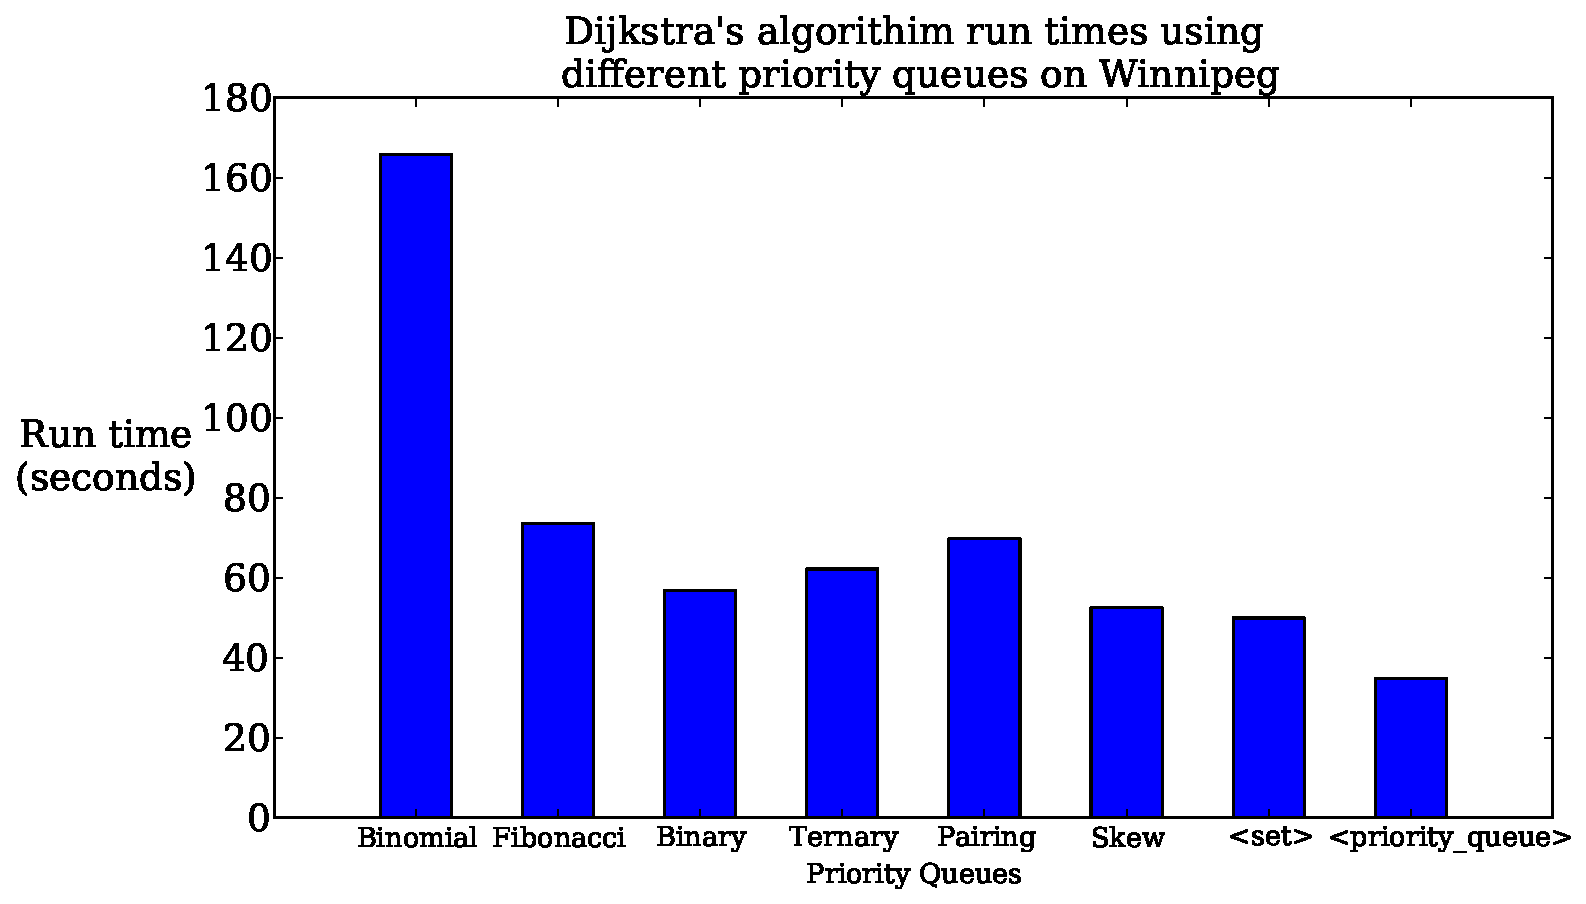
\includegraphics[page=1, width=\textwidth, height=.4\textheight]{img/pq_runtime}
    \caption{Full traffic assignment run times using Dijkstra's algorithm with different priority queues on Winnipeg, with a total number of $547{,}344$ shortest paths solved.}
    \label{fig:pq_runtime2}
\end{figure}
\begin{figure}[H]
    \centering
    \includegraphics[page=2, width=\textwidth, height=.4\textheight]{img/pq_runtime}
    \caption{Full traffic assignment run times using Dijkstra's algorithm with different priority queues on Chicago Sketch, with a total number of $2{,}328{,}375$ shortest paths solved.}
    \label{fig:pq_runtime}
\end{figure}

\section{Results on shortest path algorithms} \label{sec:allresults}
In Section~\ref{sec:pq_results} we have identified  $\langle$priority\_queue$\rangle$ to be the most suitable (efficient) data structure to be used in Dijkstra's algorithm
Now we use $\langle$priority\_queue$\rangle$, implement and test the following algorithms:
\begin{itemize}
        \item Bellman-Ford-Moore algorithm (existing),
        \item Dijkstra's algorithm,
        \item Bidirectional Dijkstra's algorithm,
        \item A* search,
        \item Bidirectional A* search.
\end{itemize}
%Therefore we use $\langle$priority\_queue$\rangle$ from the C++ standard template library and implement Dijkstra's algorithms and A* search, as well as their bidirectional versions.
Figure~\ref{fig:allresults} shows the performance of the mentioned algorithms on the Anaheim, Barcelona, Winnipeg and Chicago Sketch networks
(see Appendix~\ref{appendix:sp_results} for exact numerical results).
The networks are spaced out on the horizontal axis to show their relative sizes, i.e.\ the number of O-D pairs.

Bellman-Ford-Moore algorithm has the worst performance while the A* search has the best performance on all networks.
The bidirectional versions of Dijkstra's algorithm and A* search are more than twice slower than their unidirectional versions.

\begin{figure}[H]
    \centering
    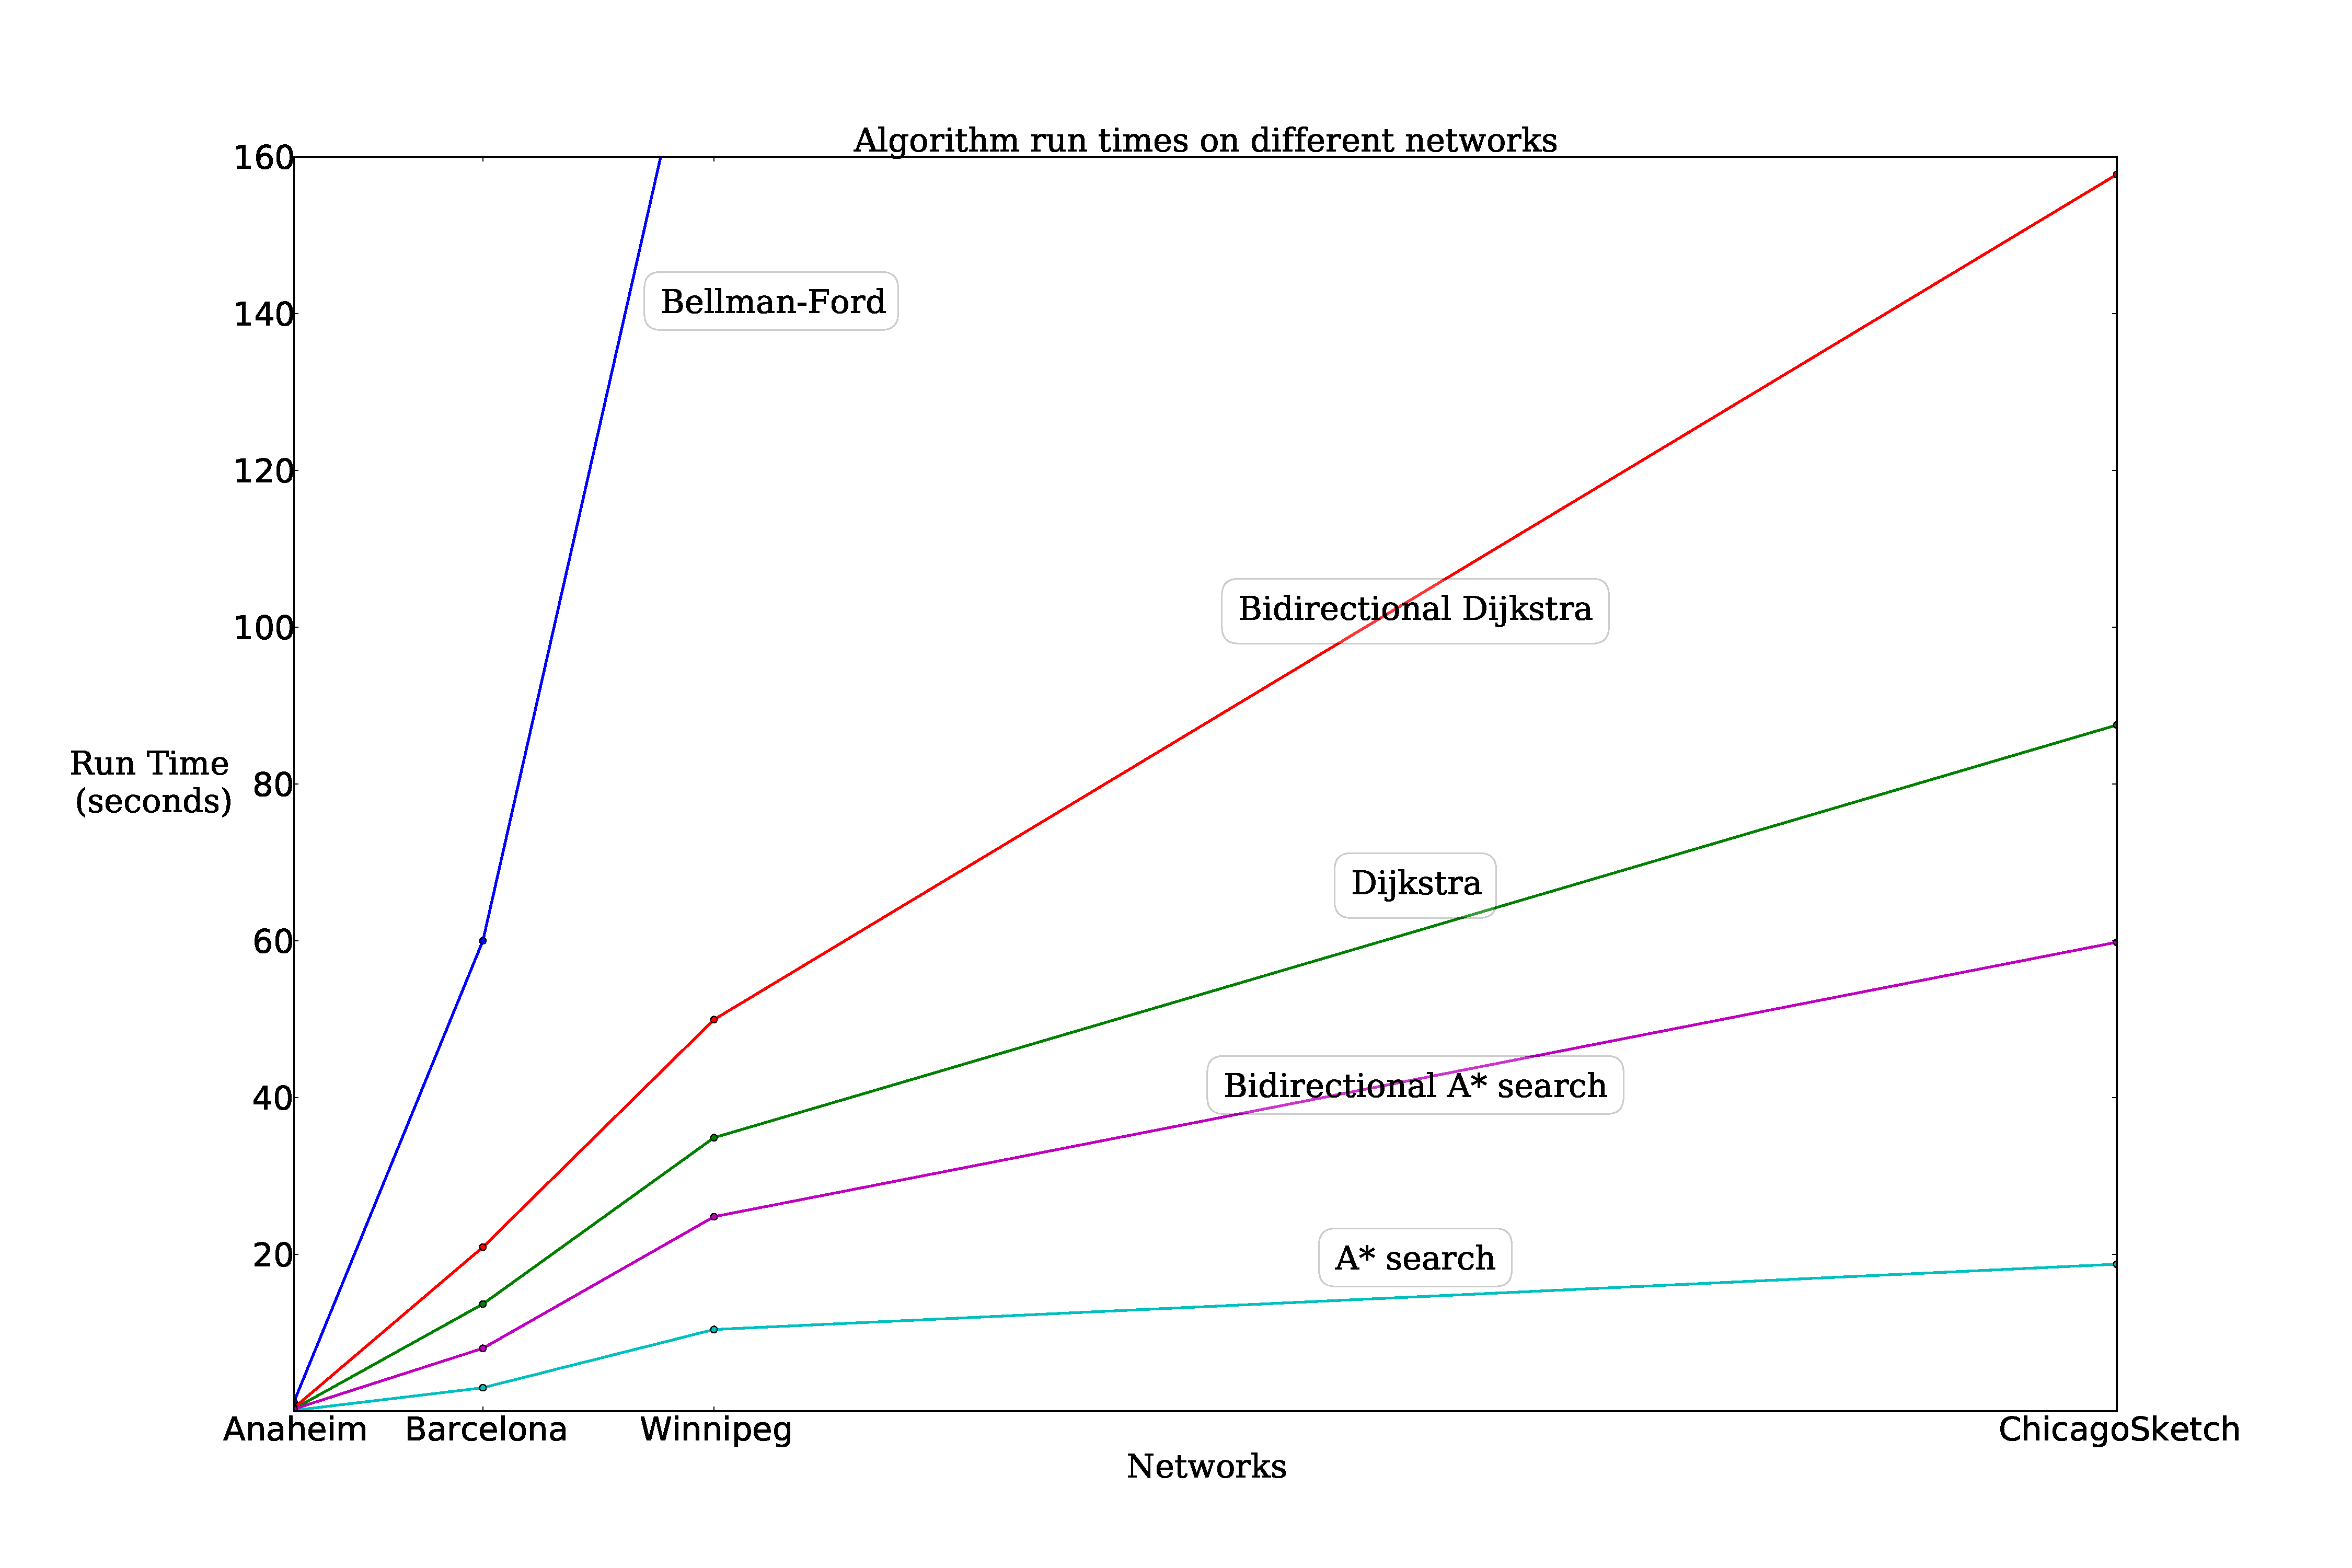
\includegraphics[width=\textwidth]{img/runtime}
    \caption{Run time performances of different algorithms on different networks}
    \label{fig:allresults}
\end{figure}
\todo[inline]{bigger axis label and remove line to different shapes}

\section{Results on avoiding shortest path calculations}
In Section~\ref{sec:allresults} we have identified A* search to be the most suitable (efficient) algorithm for solving the point-to-point shortest path problem.
In this section, we consider avoiding shortest path calculations in the iterative path equilibration algorithm discussed in Section~\ref{section:avoid}.
A* search is used to generate results for this section.

As mentioned in Section~\ref{section:avoid},
in order to apply shortest path avoiding strategies,
we need to first prove that most of the shortest paths do not change often.

Figure~\ref{fig:sp_change} shows 
the histogram for the number of times the shortest path for an O-D pair changed 0,1,2,\ldots times on the Chicago Sketch network.
It shows out of 26 iterations,
the percentage of O-D pairs that changed their shortest path once, twice, three times etc.
The figure shows that 60\% of O-D pairs have not changed their shortest path after the initial iteration,
and 16\% of O-D pairs changed their shortest path only once.
This means that after the first iterations,
the algorithm spends most of its time changing only a dozen of O-D pairs' shortest path out of $93{,}135$.
From these observations,
it is assured that run time can be reduced if we avoid shortest path calculations on the paths that do not change between iterations.

\begin{figure}[H]
    \centering
    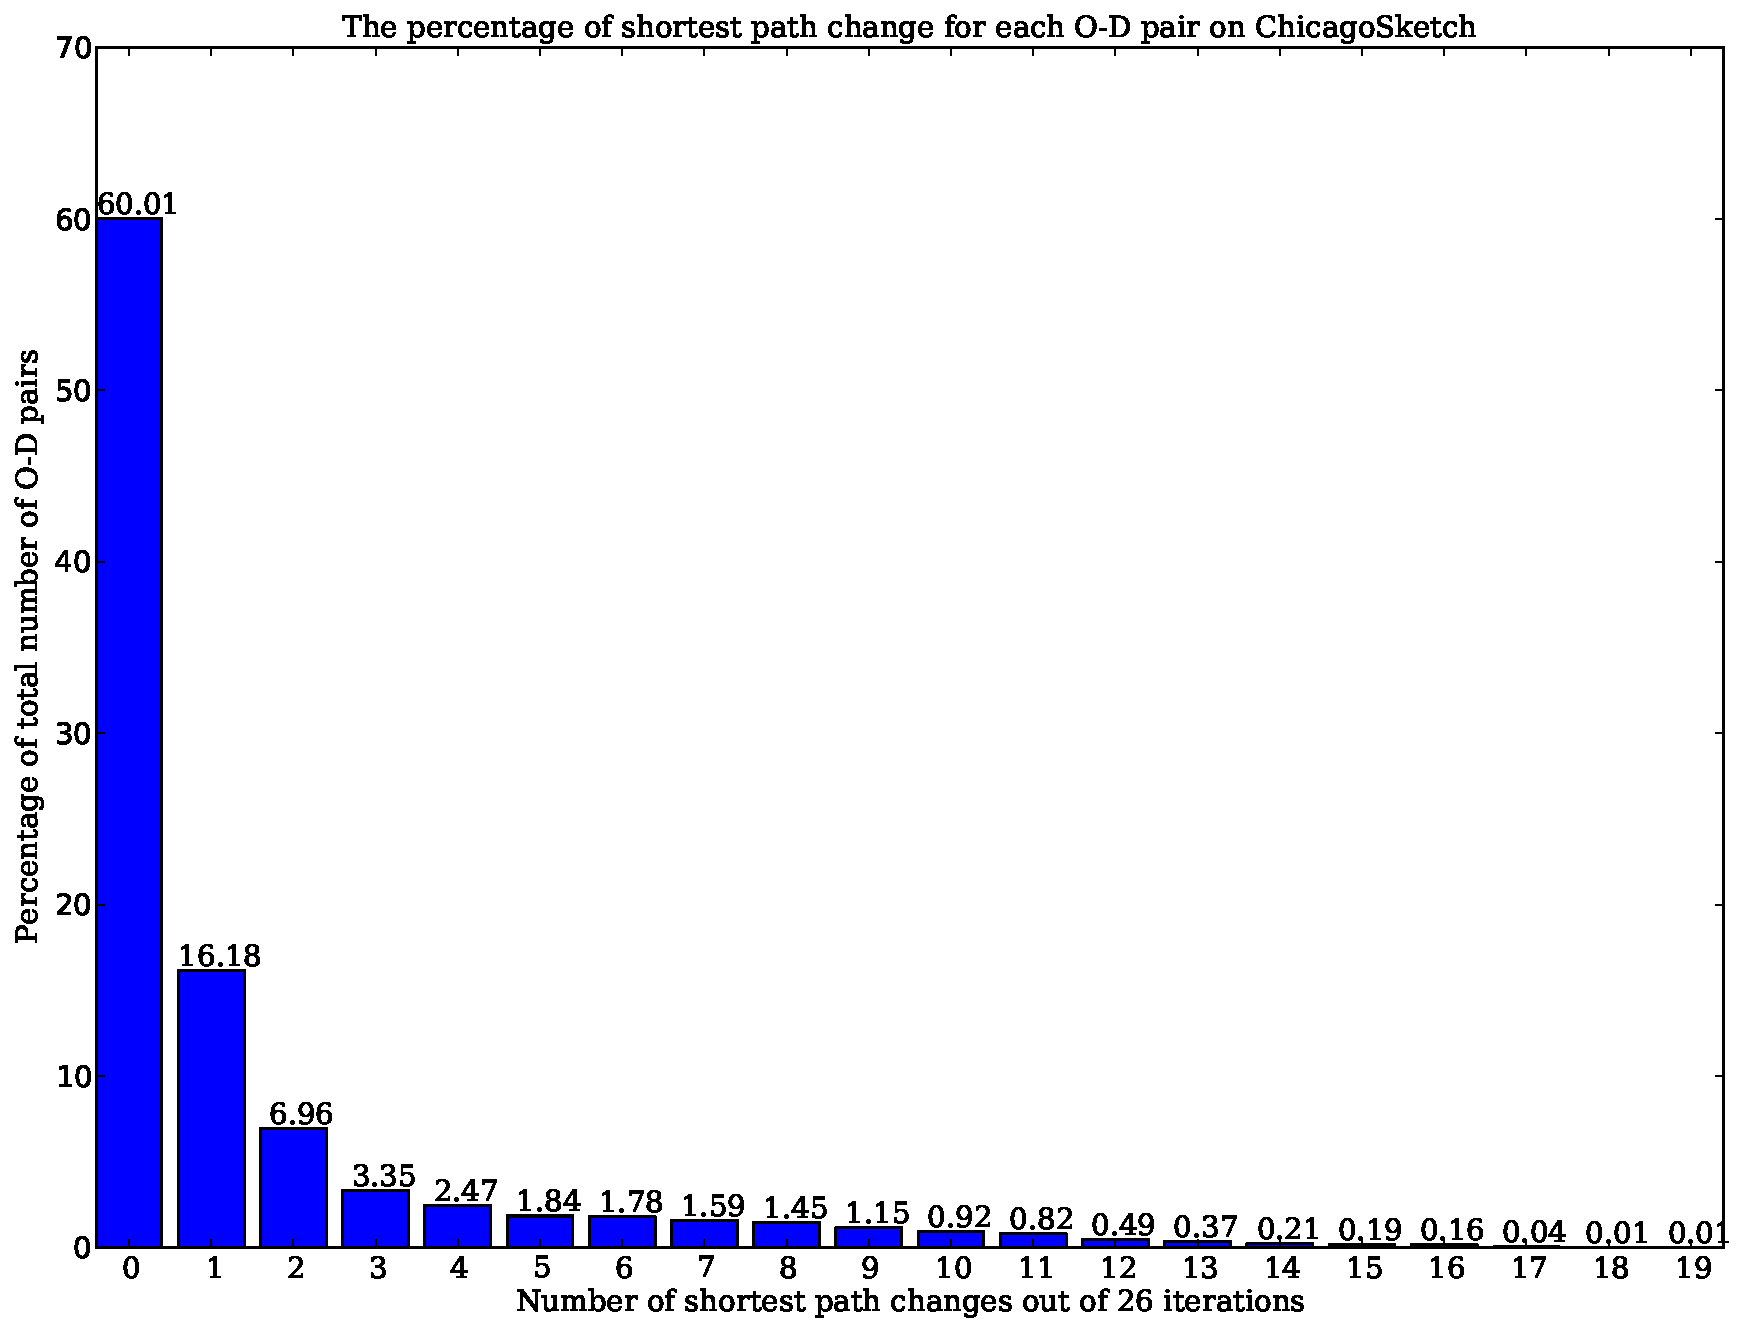
\includegraphics[page=1, height=.5\textheight]{img/sp_change}
    \caption{The percentage of shortest path change for each O-D pair out of 26 iterations for Chicago Sketch}
    \label{fig:sp_change}
\end{figure}
\begin{figure}[H]
    \centering
    \includegraphics[page=2, height=.5\textheight]{img/sp_change}
    \caption{The percentage of shortest path change for each O-D pair out of 26 iterations for Chicago Sketch}
    \label{fig:sp_change2}
\end{figure}
\todo{change title and axis label}

We now present the strategy of avoiding a pre-defined number of shortest path calculations for each O-D pair if the previous two iterations result in the identical shortest path trees.
The results are shown in Figure~\ref{fig:skip_n},
where the strategy is experimented on the Terrassa and Chicago Sketch network.
On the Terrassa network,
we choose to avoid the next 15, 25, 50, 100 and 200 iterations of shortest path calculations if the previous two are the same.
And on the Chicago Sketch network,
we choose to avoid the next 5, 10, 15 and 20 iterations.
The strategy worked well on the Terrassa network,
where run time is decreased by half for all of the chosen number of avoiding iterations.
Due to small size of the network,
the run time is not affected even though the total number of iterations increased to 563 when calculations are avoided by 200 iterations.
The strategy also worked well on the Chicago Sketch network.
Skipping 5 iterations resulted the same 26 iterations and the run time is decreased by 4 seconds.
Run times are still reduced in cases where there is an increase in total number of iterations.

\begin{figure}[H]
    \centering
    \begin{subfigure}{.5\textwidth}
        \centering
        \includegraphics[page=3,width=\textwidth]{img/random_time}
        \caption{Terrassa network}
        \label{fig:terrassa_skip_n}
    \end{subfigure}%
    \begin{subfigure}{.5\textwidth}
        \centering
        \includegraphics[page=4,width=\textwidth]{img/random_time}
        \caption{Chicago Sketch network}
        \label{fig:chicago_skip_n}
    \end{subfigure}
    \caption{Run time for avoiding shortest path calculations if the previous two iteration did not change}
    \label{fig:skip_n}
\end{figure}

The other strategy is to skip the next shortest path calculation randomly.
%The advantage of this strategy is that it does not need the number of iterations it will compute,
%but the disadvantage is that the run time may vary between different runs.
Figure~\ref{fig:terrassa_random_n} shows the results on the Terrassa network, probabilities of 0.3, 0.4, 0.5, 0.6 and 0.7 for skipping the next shortest path calculation.
The strategy reduced the run time quite significantly for all probabilities,
especially 0.5.
Figure~\ref{fig:chicago_random_n} shows effect of the same strategy on the Chicago Sketch network.
This time all run times are reduced slightly, with 0.4 having the most reduction.

\begin{figure}[H]
    \centering
    \begin{subfigure}{.5\textwidth}
        \centering
        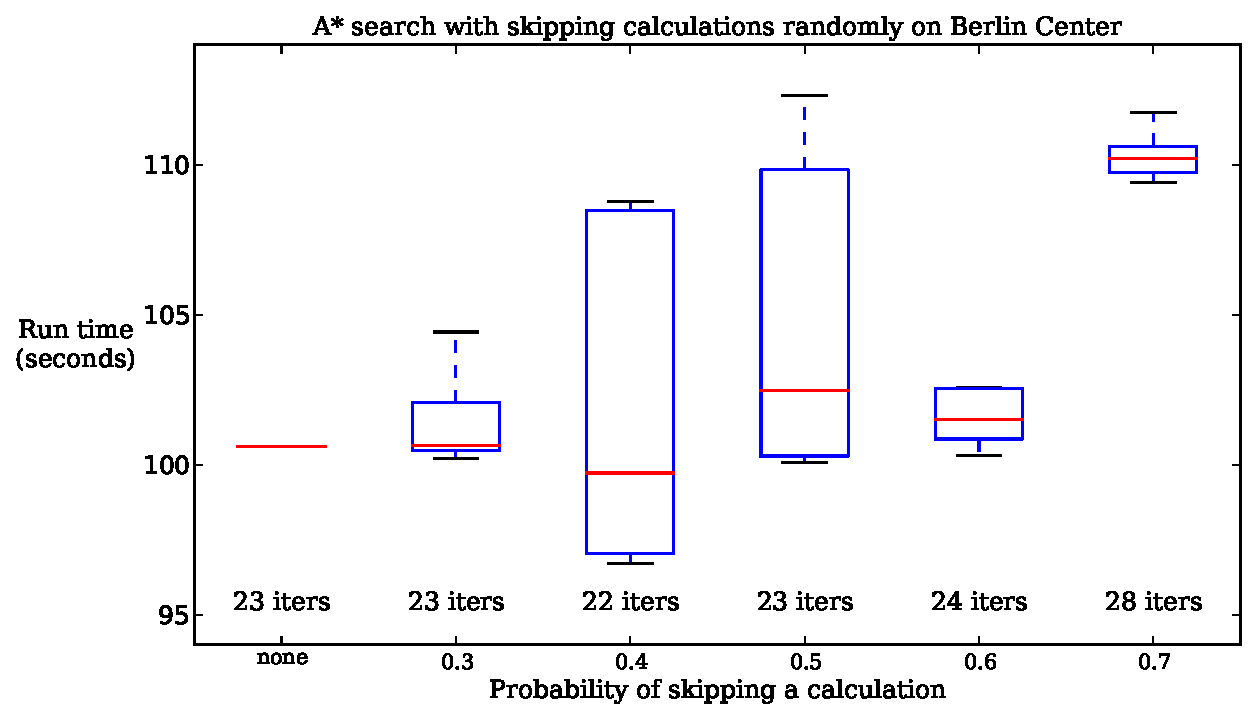
\includegraphics[page=1,width=\textwidth]{img/random_time}
        \caption{Terrassa network}
        \label{fig:terrassa_random_n}
    \end{subfigure}%
    \begin{subfigure}{.5\textwidth}
        \centering
        \includegraphics[page=2,width=\textwidth]{img/random_time}
        \caption{ChicagoSketch network}
        \label{fig:chicago_random_n}
    \end{subfigure}
    \caption{Run time for skipping shortest path calculations randomly}
    \label{fig:random_n}
\end{figure}

The random strategy can be used before knowing the total number of iterations the path equilibration algorithm going to produce,
Since only small networks have been tested so far,
we now present the random strategy on the Philadelphia and Chicago Regional networks, where they have over a million number of O-D pairs.
The run time comparisons are shown in Table~\ref{table:runtime_large_network},
where the random skipping strategy uses 50\% probability to skip a shortest path calculation.
The strategy has a 25\% and 27\% run time improvement on the Philadelphia and Chicago Regional networks respectively.

\begin{table}[H]
    \begin{tabular*}{\textwidth}{@{\extracolsep{\fill}} l | c c}
        & Philadelphia & Chicago Regional \\ \midrule
        A* search & 7.69 hours & 33.26 hours \\ 
        A* search with 50\% random skipping & 5.75 hours & 24.18 hours\\
    \end{tabular*}
    \caption{Run time of A* search and the randomly skipping strategy on Philadelphia and Chicago Regional network}
    \label{table:runtime_large_network}
\end{table}

\todo[inline]{see page 34 Andrea fix}


\newpage
\chapter{Further discussions}
The previous chapter presented results that indicated A* search using priority queue from the C++ standard template library has the best performance.
The results also shows that shortest path calculations can be speed up further when it is in an iterative environment.
In this chapter we discuss the details behind the mentioned results,
including why some of the algorithms that should have performed better but failed to do so.

\section{Priority queues}
The priority queue implementation results showed that
all of the heap implementations from the Boost library is worse than $\langle$priority\_queue$\rangle$.
The reason behind this can be explained using the Binary heap implementation.
It turns out that the implementation of $\langle$priority\_queue$\rangle$ is almost similar to Binary heap from the Boost library,
the only difference is their underlying storage of node information.
Nodes are stored using an array in the standard library version,
where as the Boost library uses pointers to keep track of 
the nodes.
Due to computer cache coherence,
it is known that accessing data from a nearby memory (RAM) locations in a short period of time is faster than accessing from distant memory locations.
This is due to cache memory access being much faster than RAM access,
and internally a block of memory are pre-fetched into the cache in a hope they will be accessed in a short period of time).
In the shortest path algorithms,
the Heap tree need to be searched over and over in a short period of time when nodes are being scanned and inserted.
The standard library version uses an array where data are stored linearly in a nearby location,
so it is much faster than the pointer based version where memory are allocated in random locations when nodes are inserted.

\subsection{Fibonacci heap}
Here we discuss the reason behind Fibonacci heap not performing well despite its $O(1)$ amortized time Decrease-Key operation.
As described in the two priority queue sections (Section~\ref{sec:pq} and \ref{sec:pq_implementation}),
the Decrease-Key operation is used to change the distance label of a node when the node is already in the heap.
It was discovered that the $O(1)$ time has a very high constant factor,
and Fibonacci heap only works well if the underlying graph is large and dense (i.e.\ every node connects to almost every other node).
This discovery comes from the fact that 
the Decrease-Key operation is only used frequent when the graph is dense,
so cumulatively its high constant $O(1)$ time will perform better compared to $O(\log(N))$ time in other heap implementations, where $N$ need to be a large number.

Now we confirm our graph is indeed not dense and the Decrease-Key is not used frequent.
We find that all of our graphs are very sparse.
The degree of any node of any graph is no more than 5,
as it is already really rare to have an intersection with 5 roads connected.
The graphs only have about 0.4\% to 0.6\% of arcs in the corresponding complete graph (every node connects to every other node).
We also find that in all of the experimented graphs when using Dijkstra's algorithm,
the probability of using Decrease-Key on any node is around 1 to 5 percent.

\section{Bidirectional algorithms}
In this section we investigate the reason for the worse performances of the bidirectional algorithms. 

First we examine whether search areas of the algorithms are what is expected.
Figure~\ref{fig:long_sptree} shows the shortest path trees of the point-to-point algorithms, where the origin and destination node is placed on the opposite side of the ChicagoSketch network.
It can be seen that Dijkstra's algorithm scans the entire network.
Bidirectional Dijkstra scans almost the entire network with some nodes on the side left out.
Bidirectional A* scans a slightly larger region near the origin and destination nodes,
and the A* search scans just a few nodes along the shortest path.
The behaviour of the algorithms is shown further in Figure~\ref{fig:short_sptree},
where the origin and destination is placed close to each other.
It is shown that both Dijkstra's algorithm and its bidirectional version scan almost half of the graph,
where bidirectional search scans less.
A* and its bidirectional search scan a small portion of the graph,
and they do not scan the area behind the origin and destination node compared to the Dijkstra's algorithm.

The search areas of the Dijkstra's algorithms match what is expected,
but not the run times.
The reason for reduction in run time is due to our implementations.
In both forward and backward search,
the current shortest path $\mu$ need to be updated every time a node is scanned,
and the stopping criterion need to be checked when a node is labelled.
Furthermore,
once the algorithm terminates,
we need to retrieve the shortest path in both directions by following their predecessors and concatenate them together for the full shortest.
So it is concluded that these addition computations slowed down the run times.

For A* search,
the bidirectional version scans more nodes than the unidirectional version.
And since the bidirectional version has similar stopping criterion compared to the bidirectional Dijkstra's algorithm,
it is easy to understand why bidirectional A* performed worse.

\begin{figure}
    \centering
    \begin{subfigure}{.5\textwidth}
        \centering
        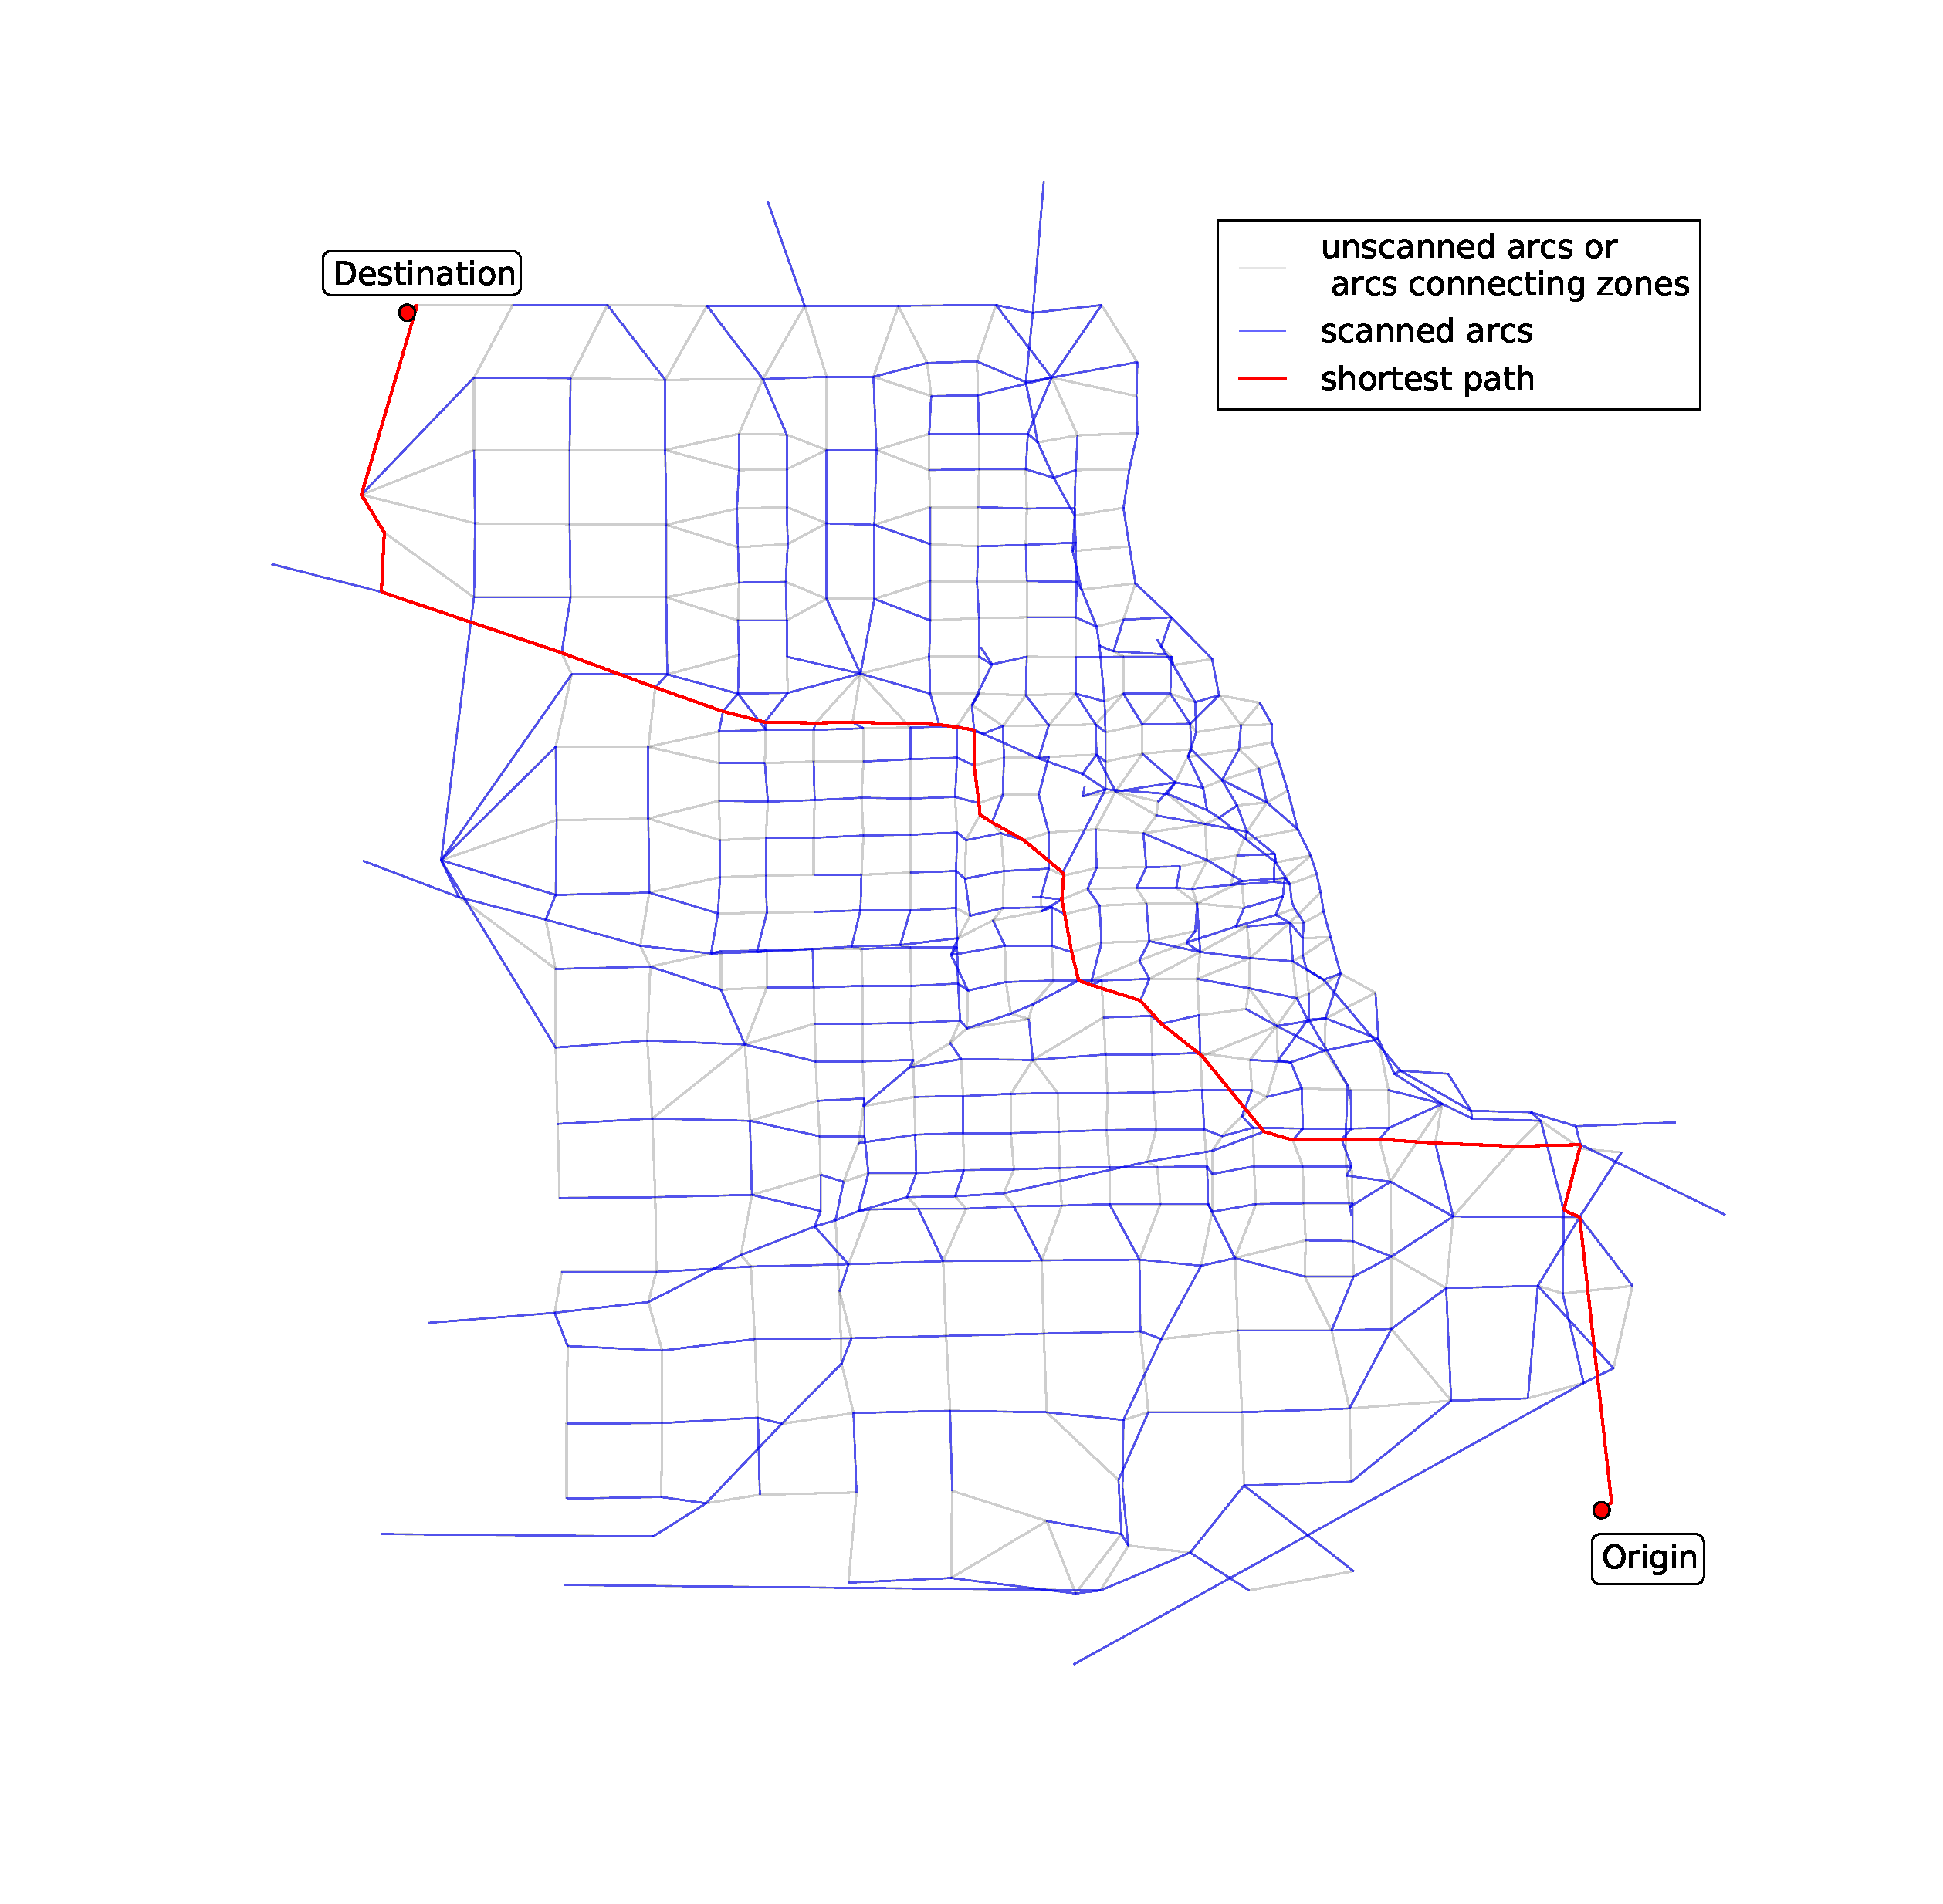
\includegraphics[width=\textwidth,trim=120px 120px 48px 120px,clip]{img/chicago_dijkstra}
        \caption{Dijkstra}
        \label{fig:chicago_dijkstra}
    \end{subfigure}%
    \begin{subfigure}{.5\textwidth}
        \centering
        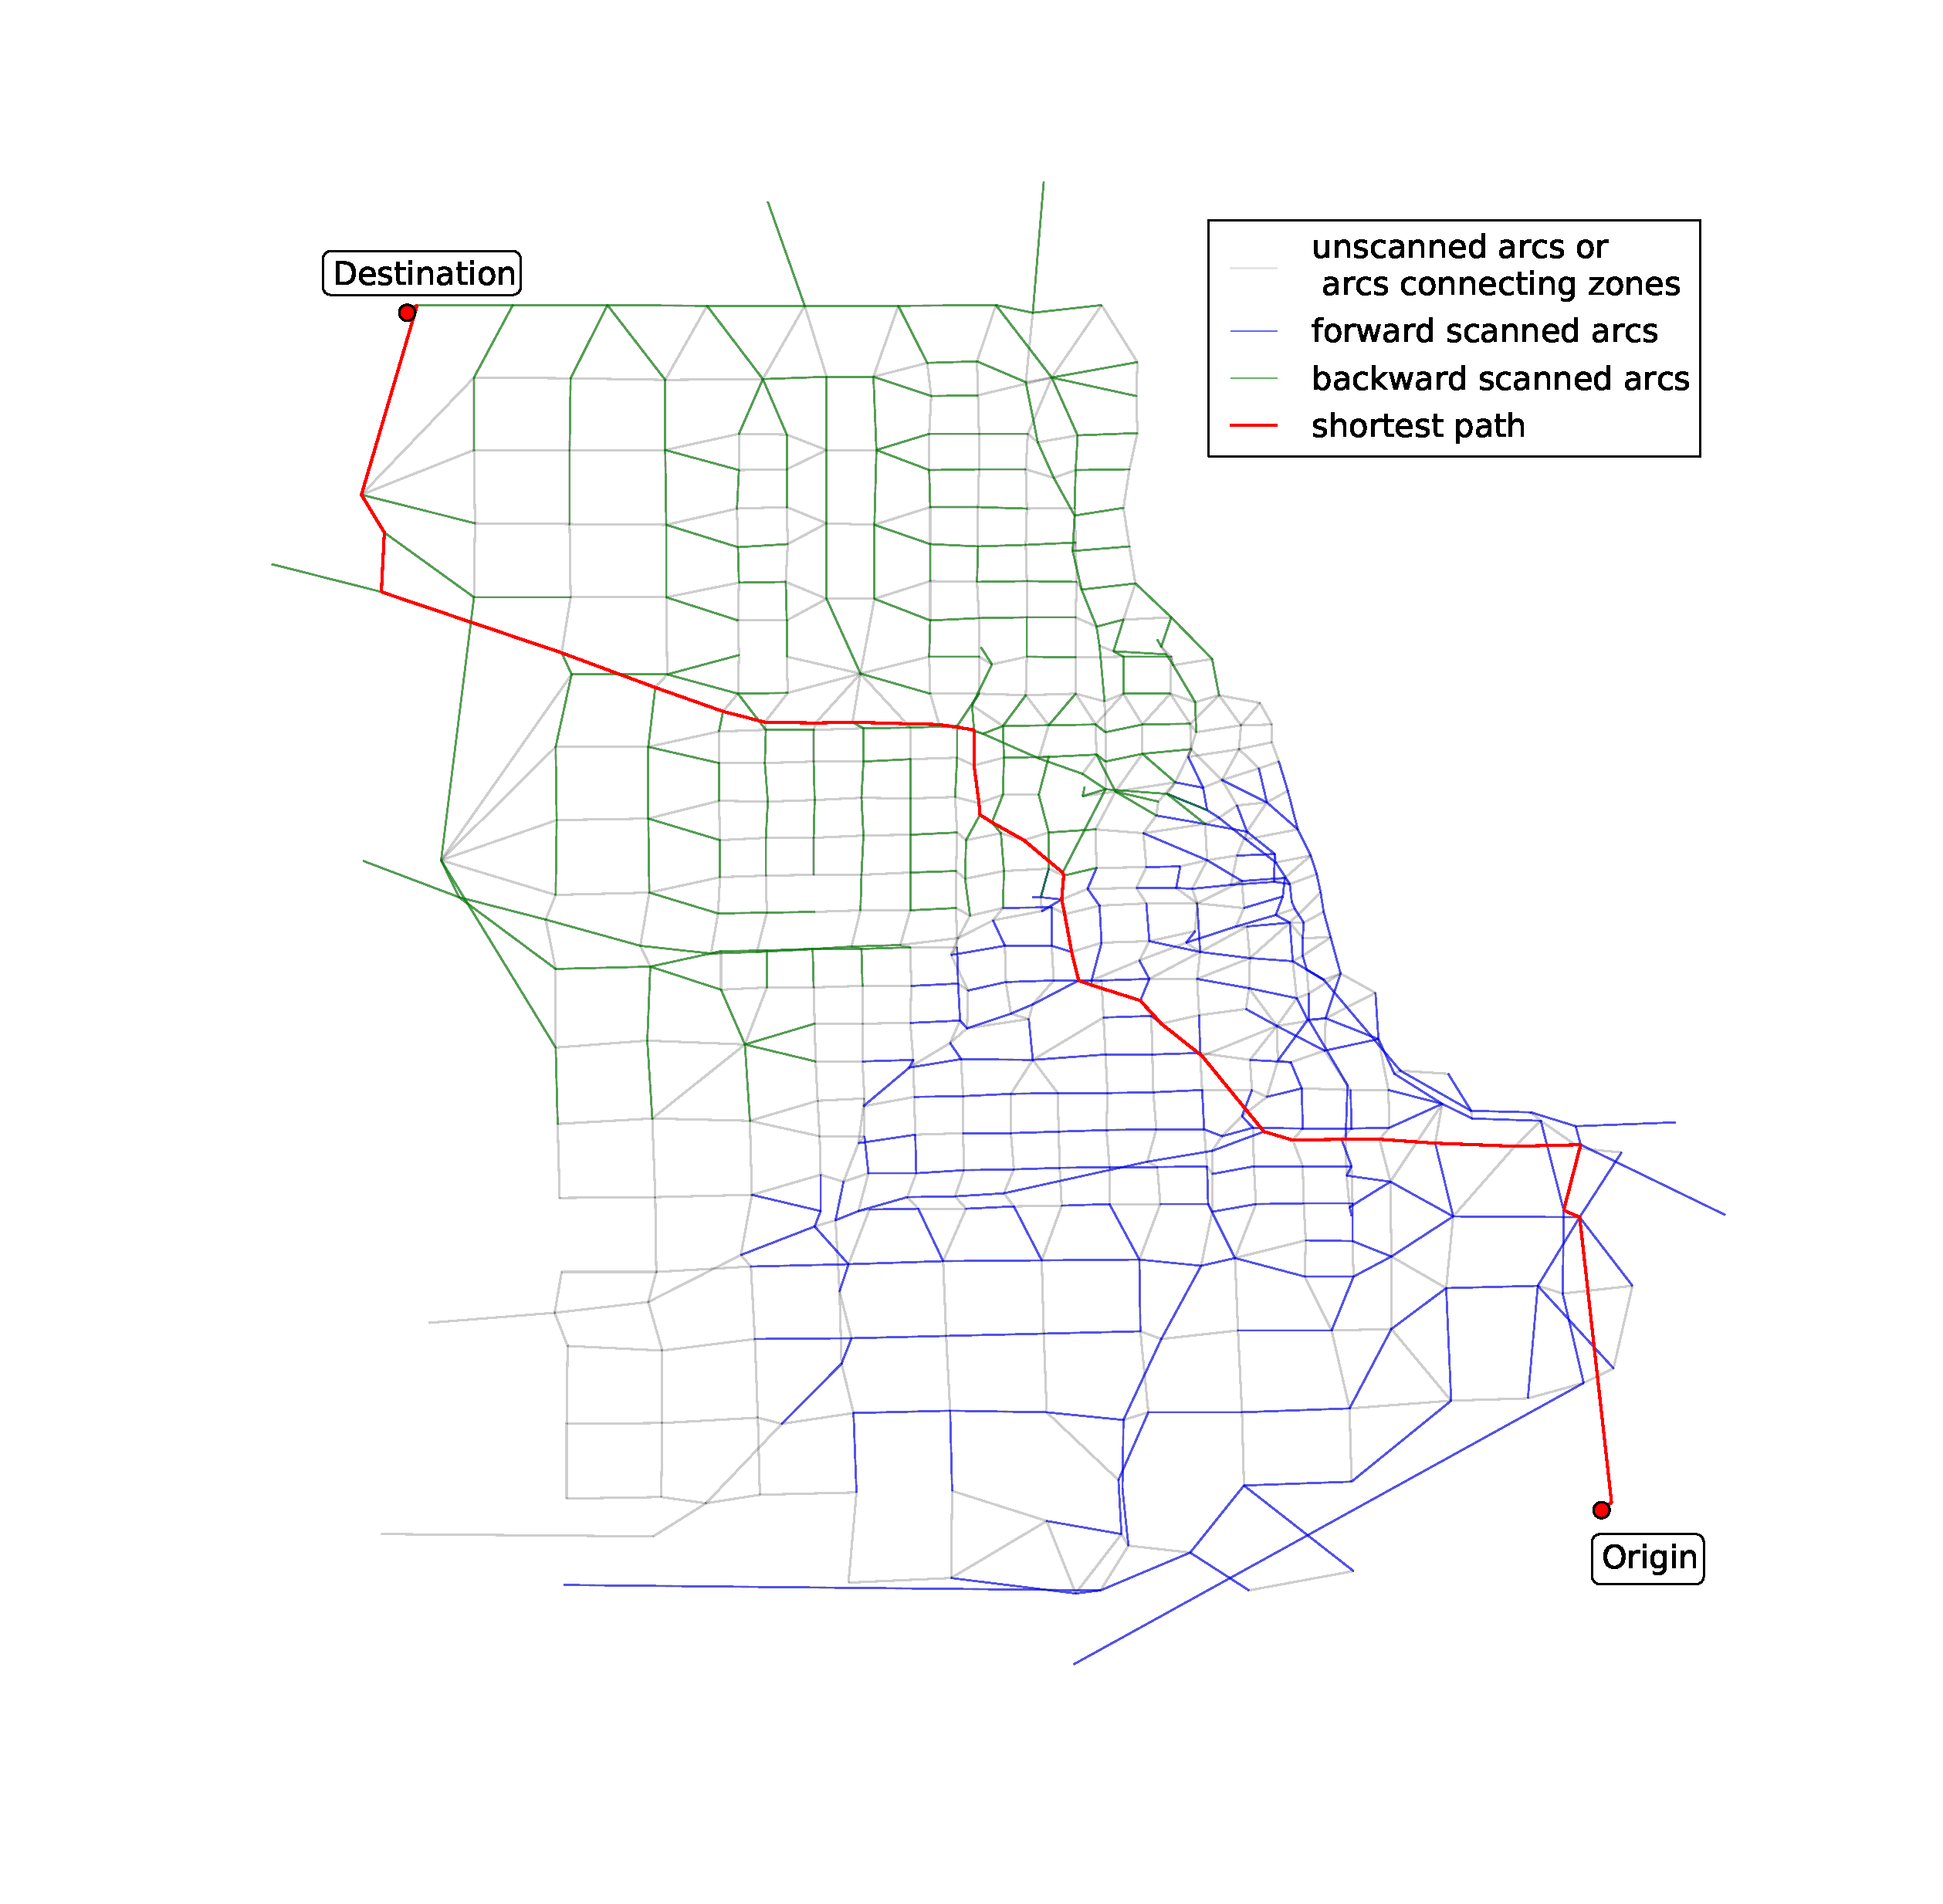
\includegraphics[width=\textwidth,trim=120px 120px 48px 120px,clip]{img/chicago_bidirect}
        \caption{Bidirectional Dijkstra}
        \label{fig:chicago_bidirect}
    \end{subfigure}
    \begin{subfigure}{.5\textwidth}
        \centering
        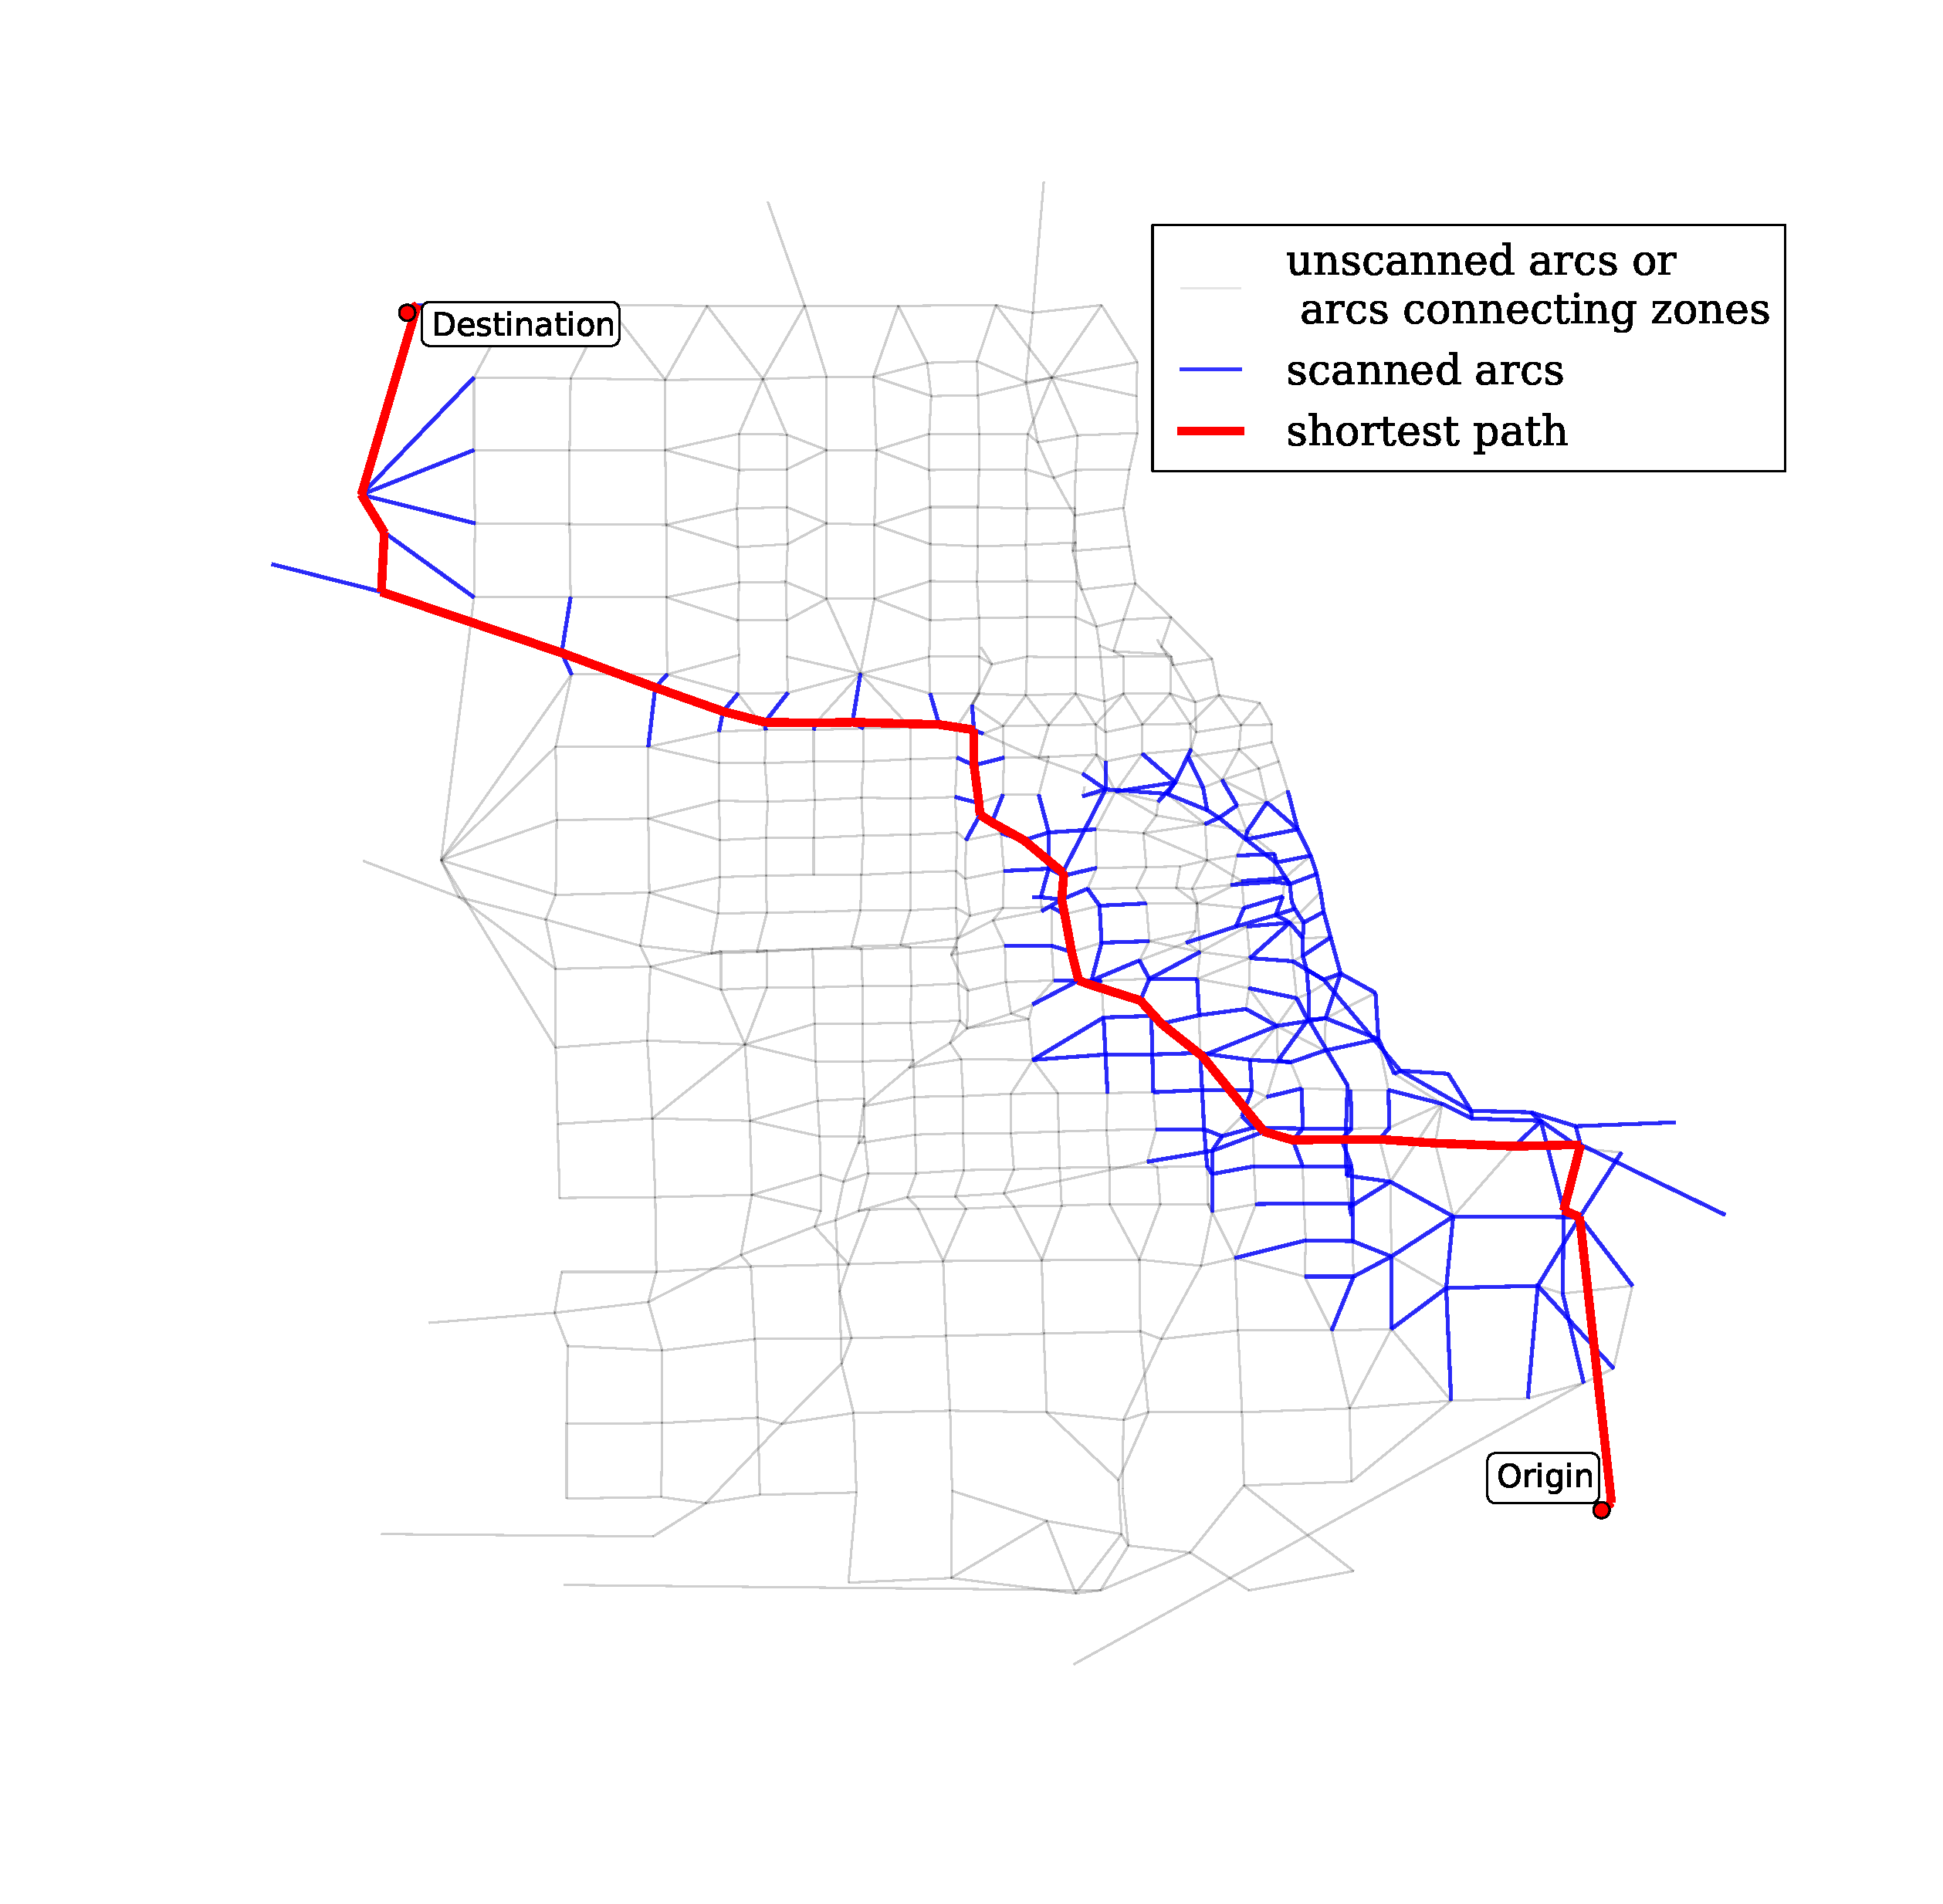
\includegraphics[width=\textwidth,trim=120px 120px 48px 0px,clip]{img/chicago_astar}
        \caption{A* Search}
        \label{fig:chicago_astar}
    \end{subfigure}%
    \begin{subfigure}{.5\textwidth}
        \centering
        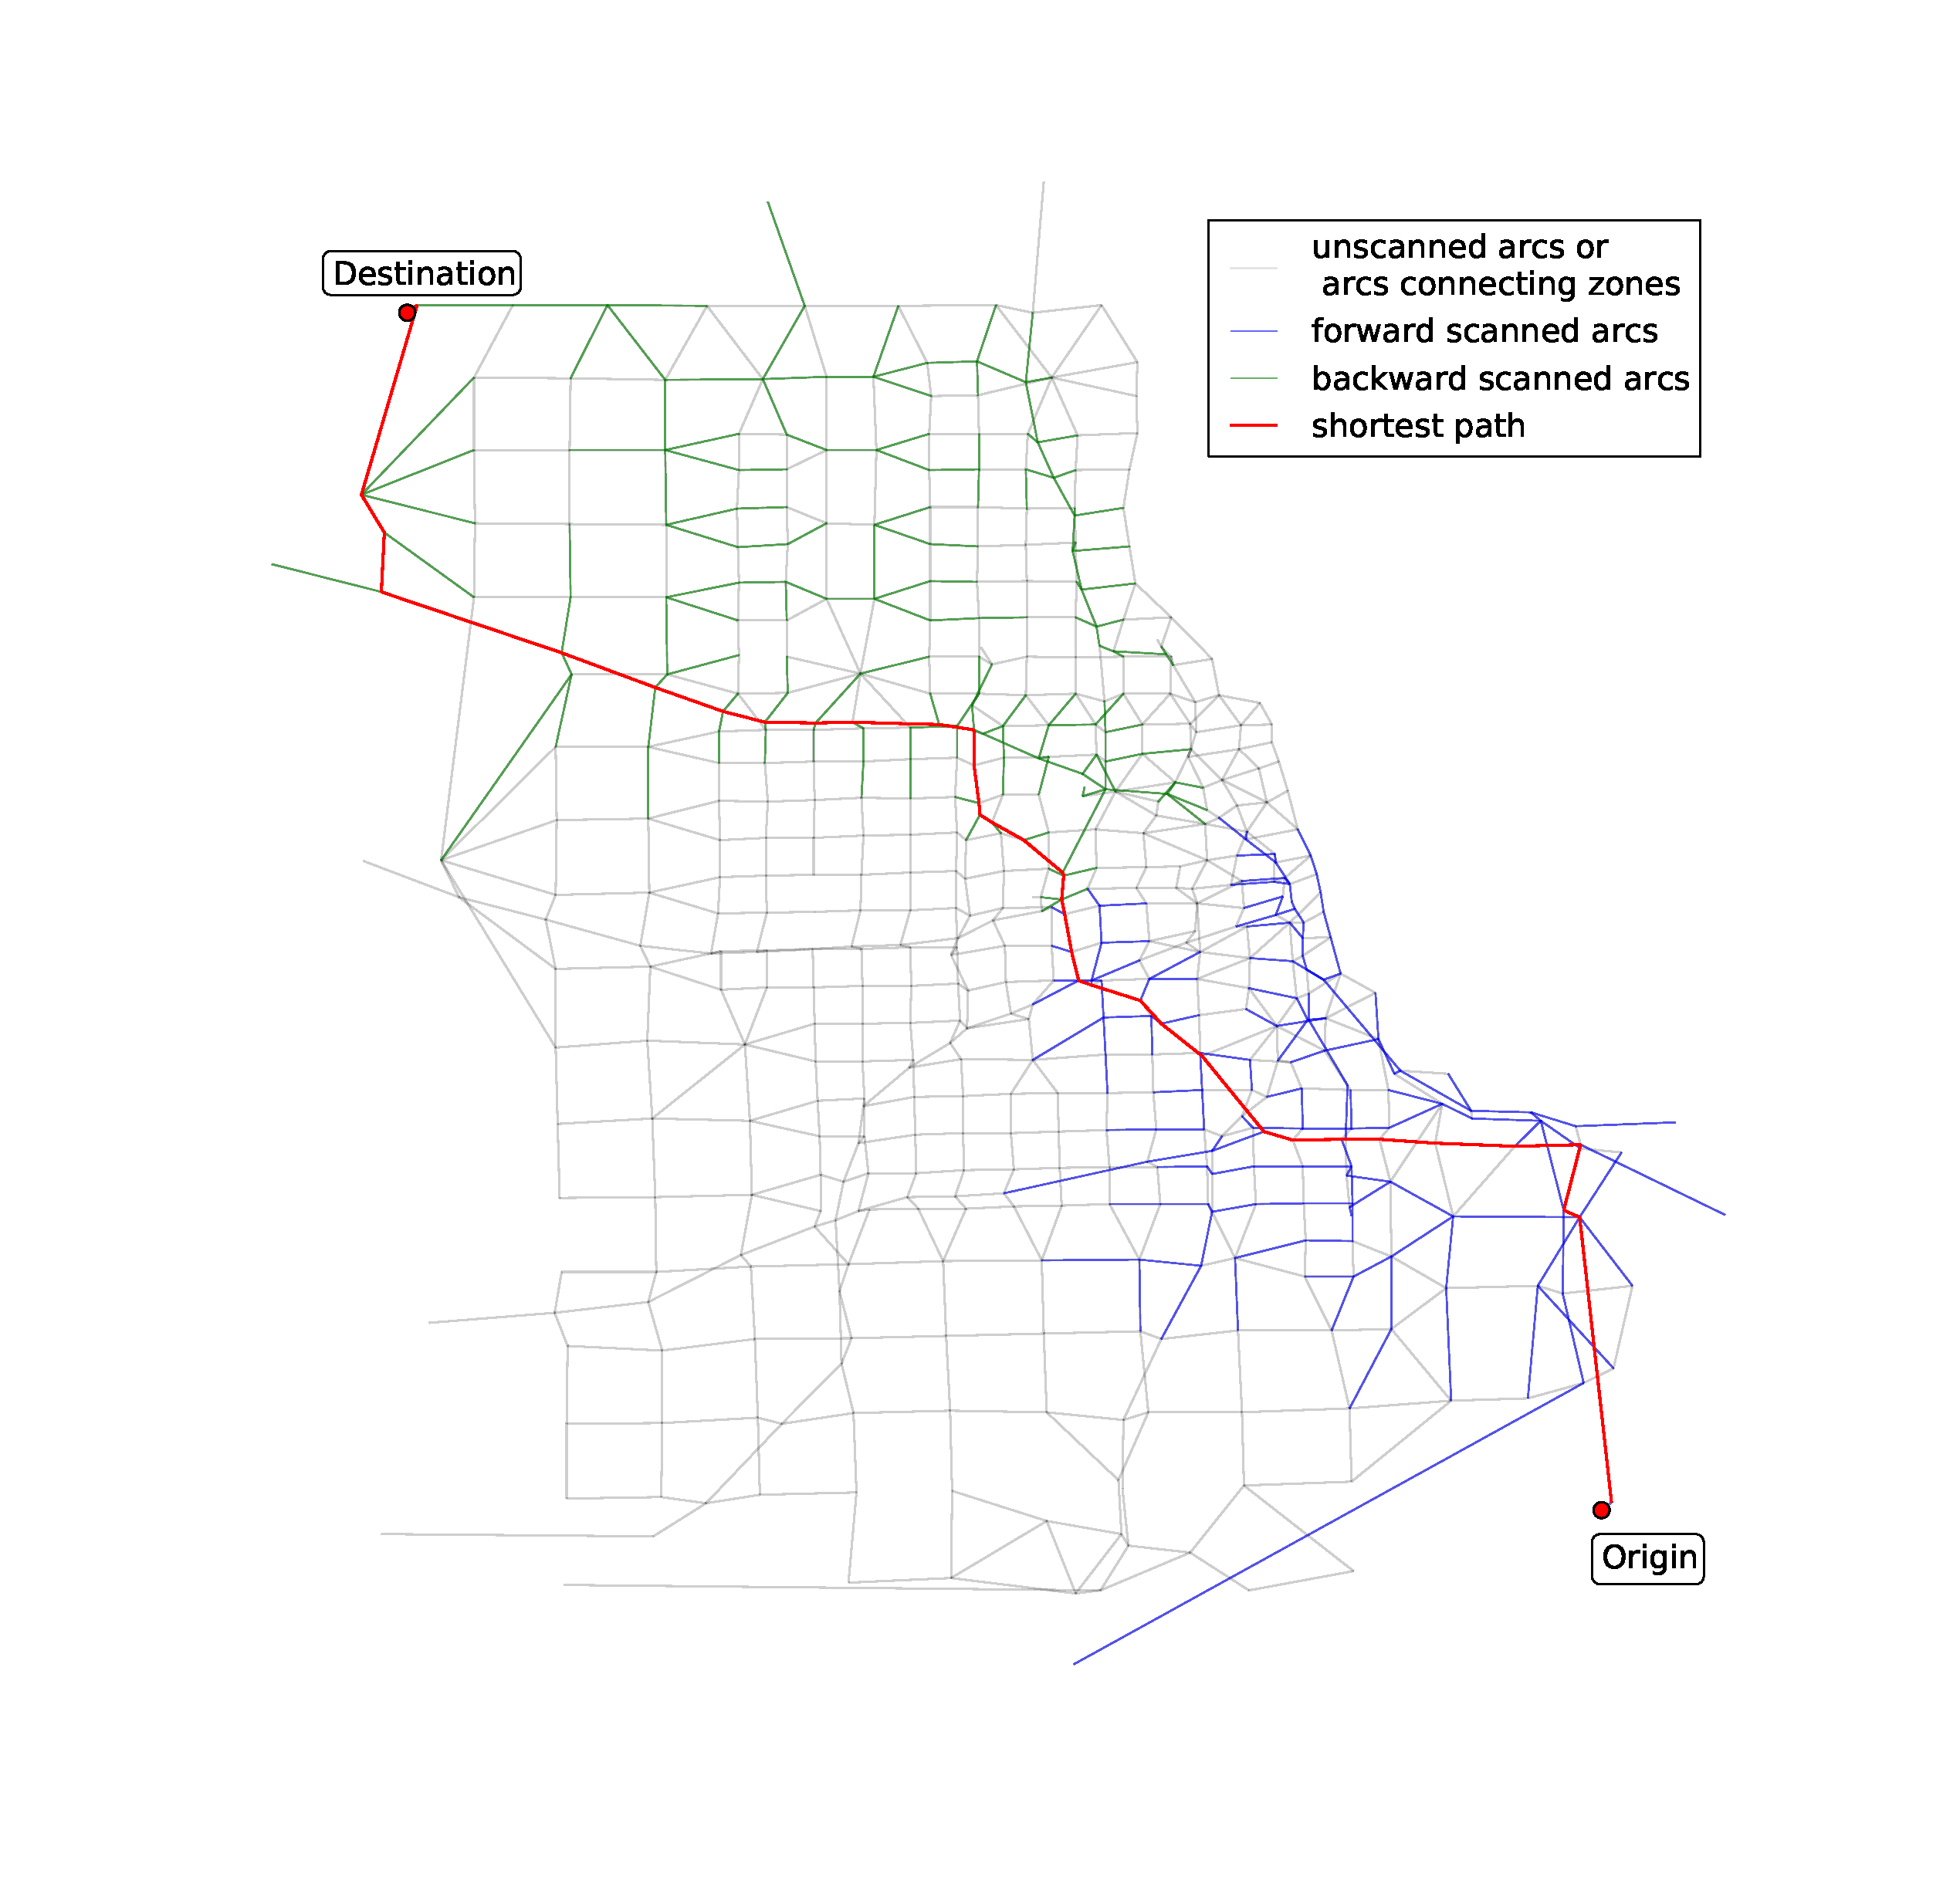
\includegraphics[width=\textwidth,trim=120px 120px 48px 0px,clip]{img/chicago_astar_bidirect}
        \caption{Bidirectional A* Search}
        \label{fig:chicago_astar_bidirect}
    \end{subfigure}
    \vspace{1em}
    \caption{Shortest path tree between two distant nodes in the ChicagoSketch Network}
    \label{fig:long_sptree}
\end{figure}

\begin{figure}
    \centering
    \begin{subfigure}{.5\textwidth}
        \centering
        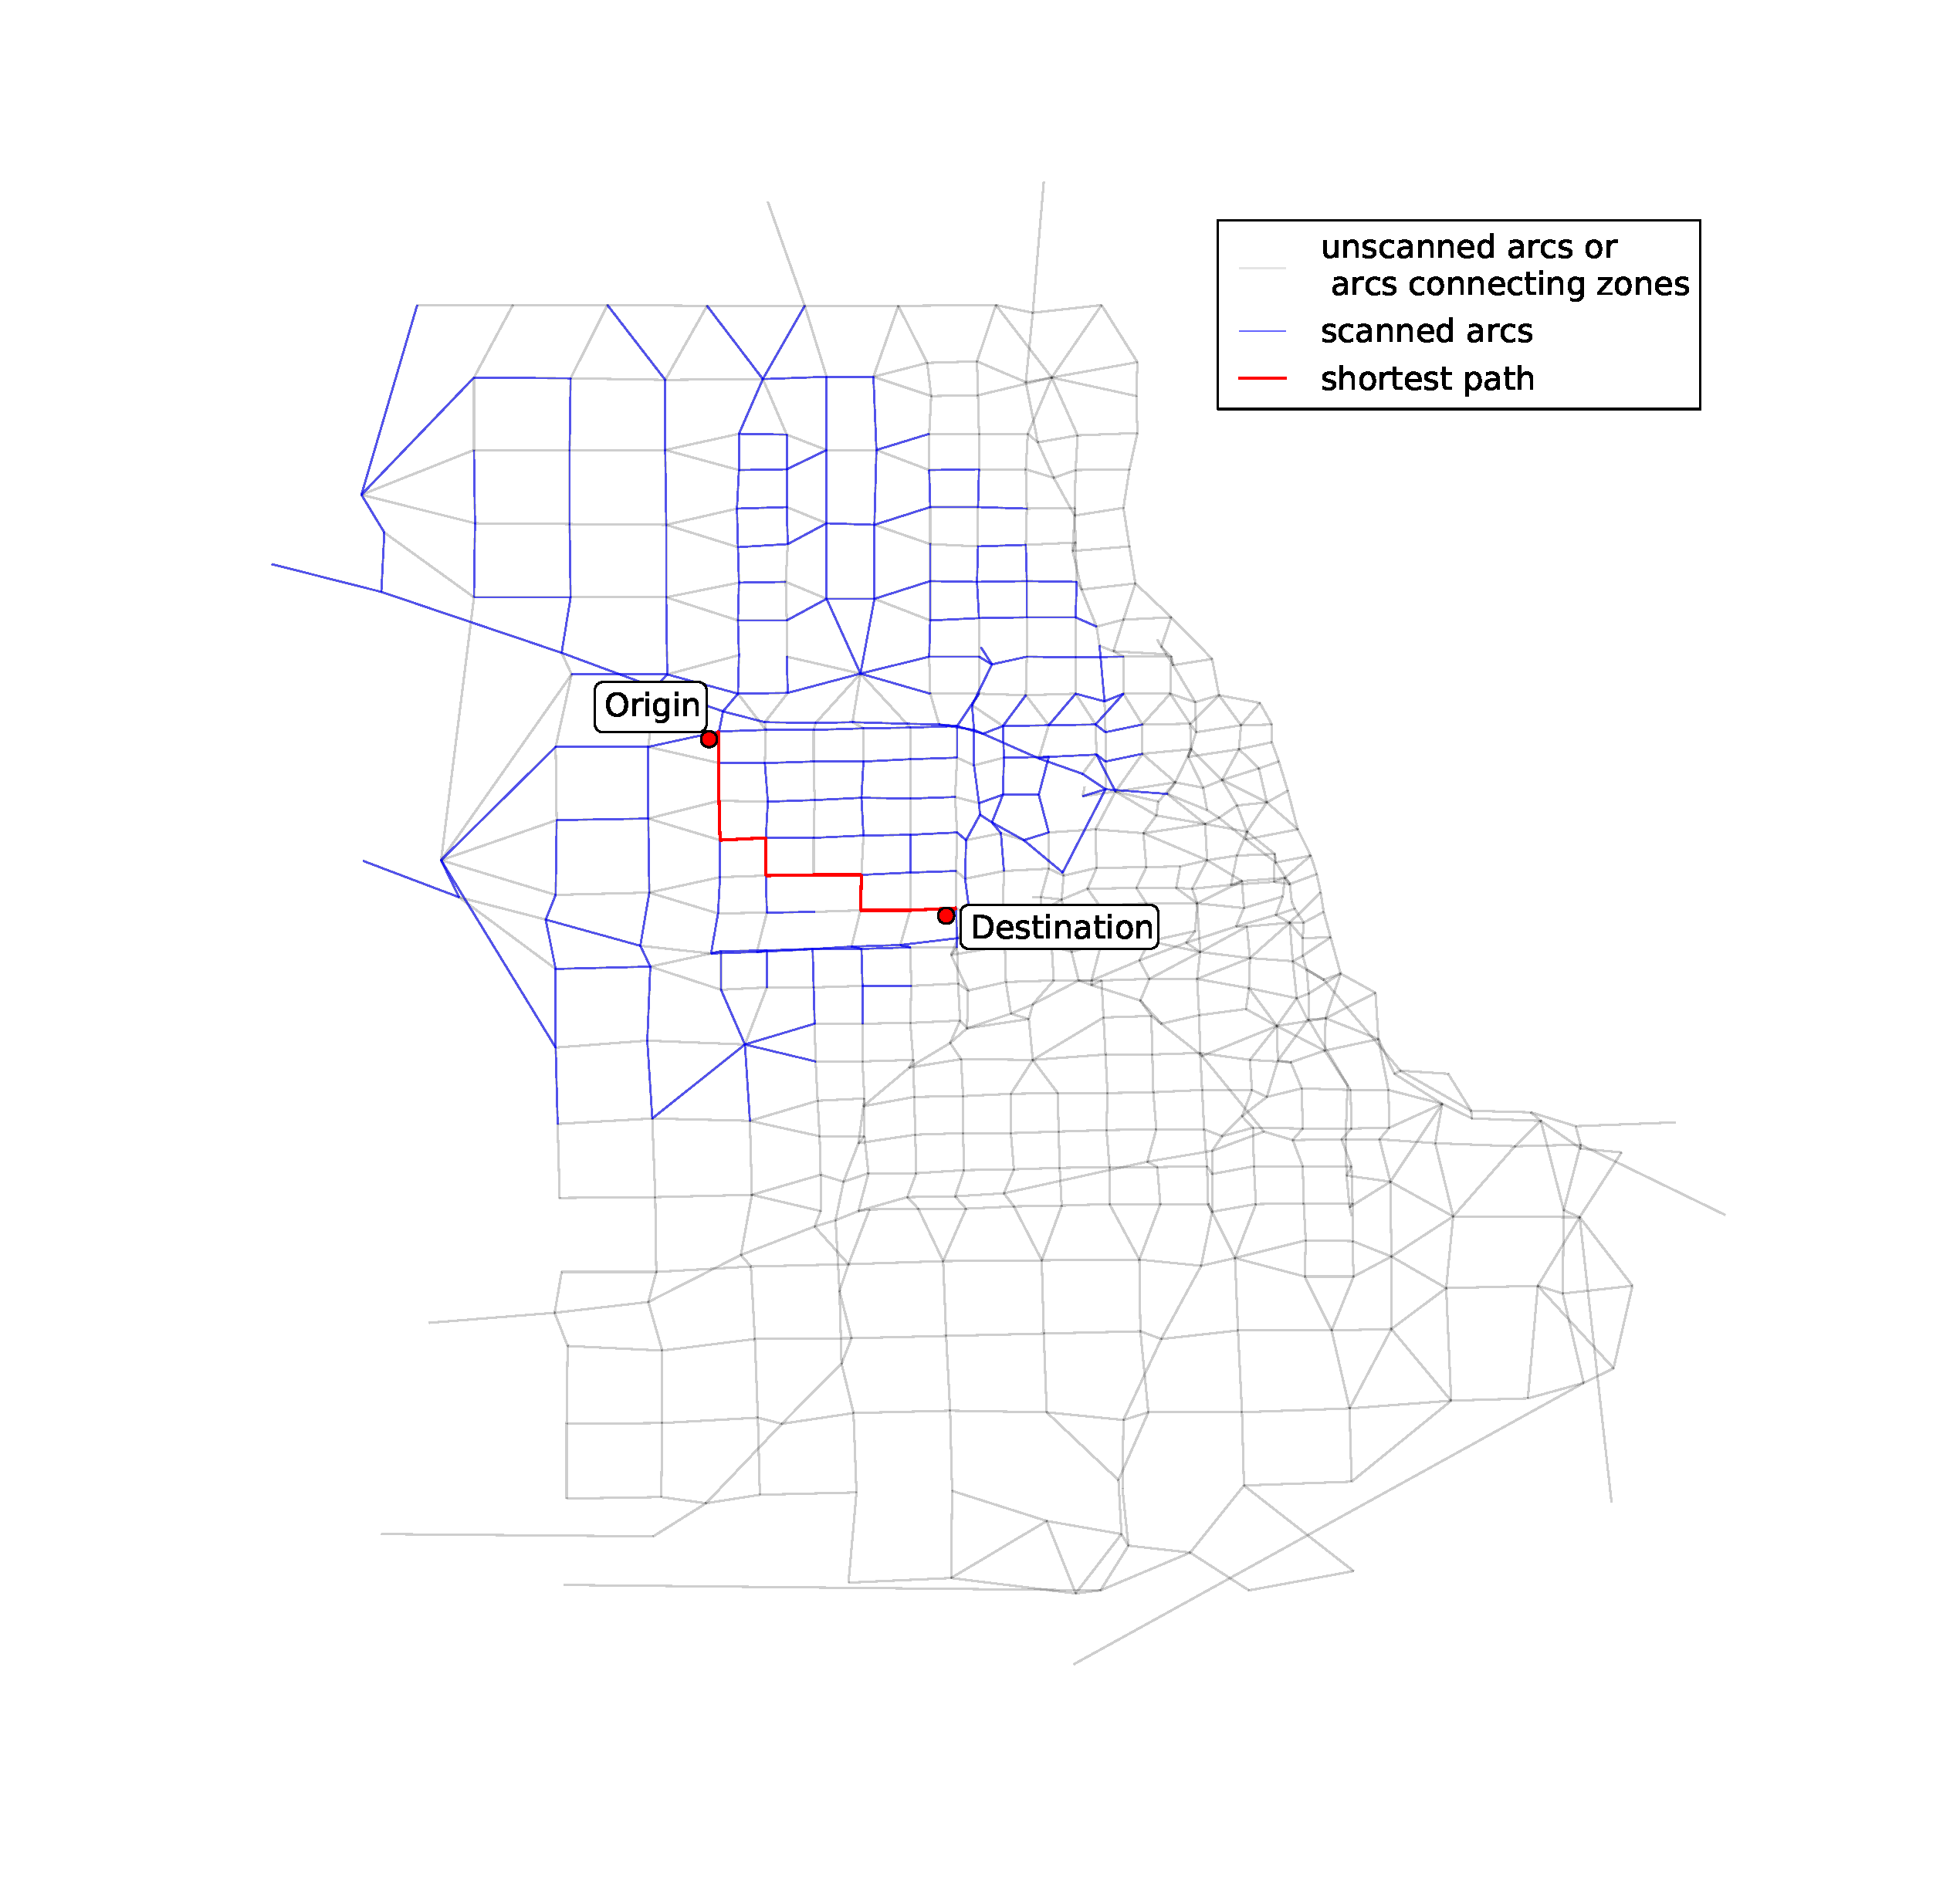
\includegraphics[width=\textwidth,trim=120px 120px 48px 120px,clip]{img/chicago_dijkstra2}
        \caption{Dijkstra}
        \label{fig:chicago_dijkstra2}
    \end{subfigure}%
    \begin{subfigure}{.5\textwidth}
        \centering
        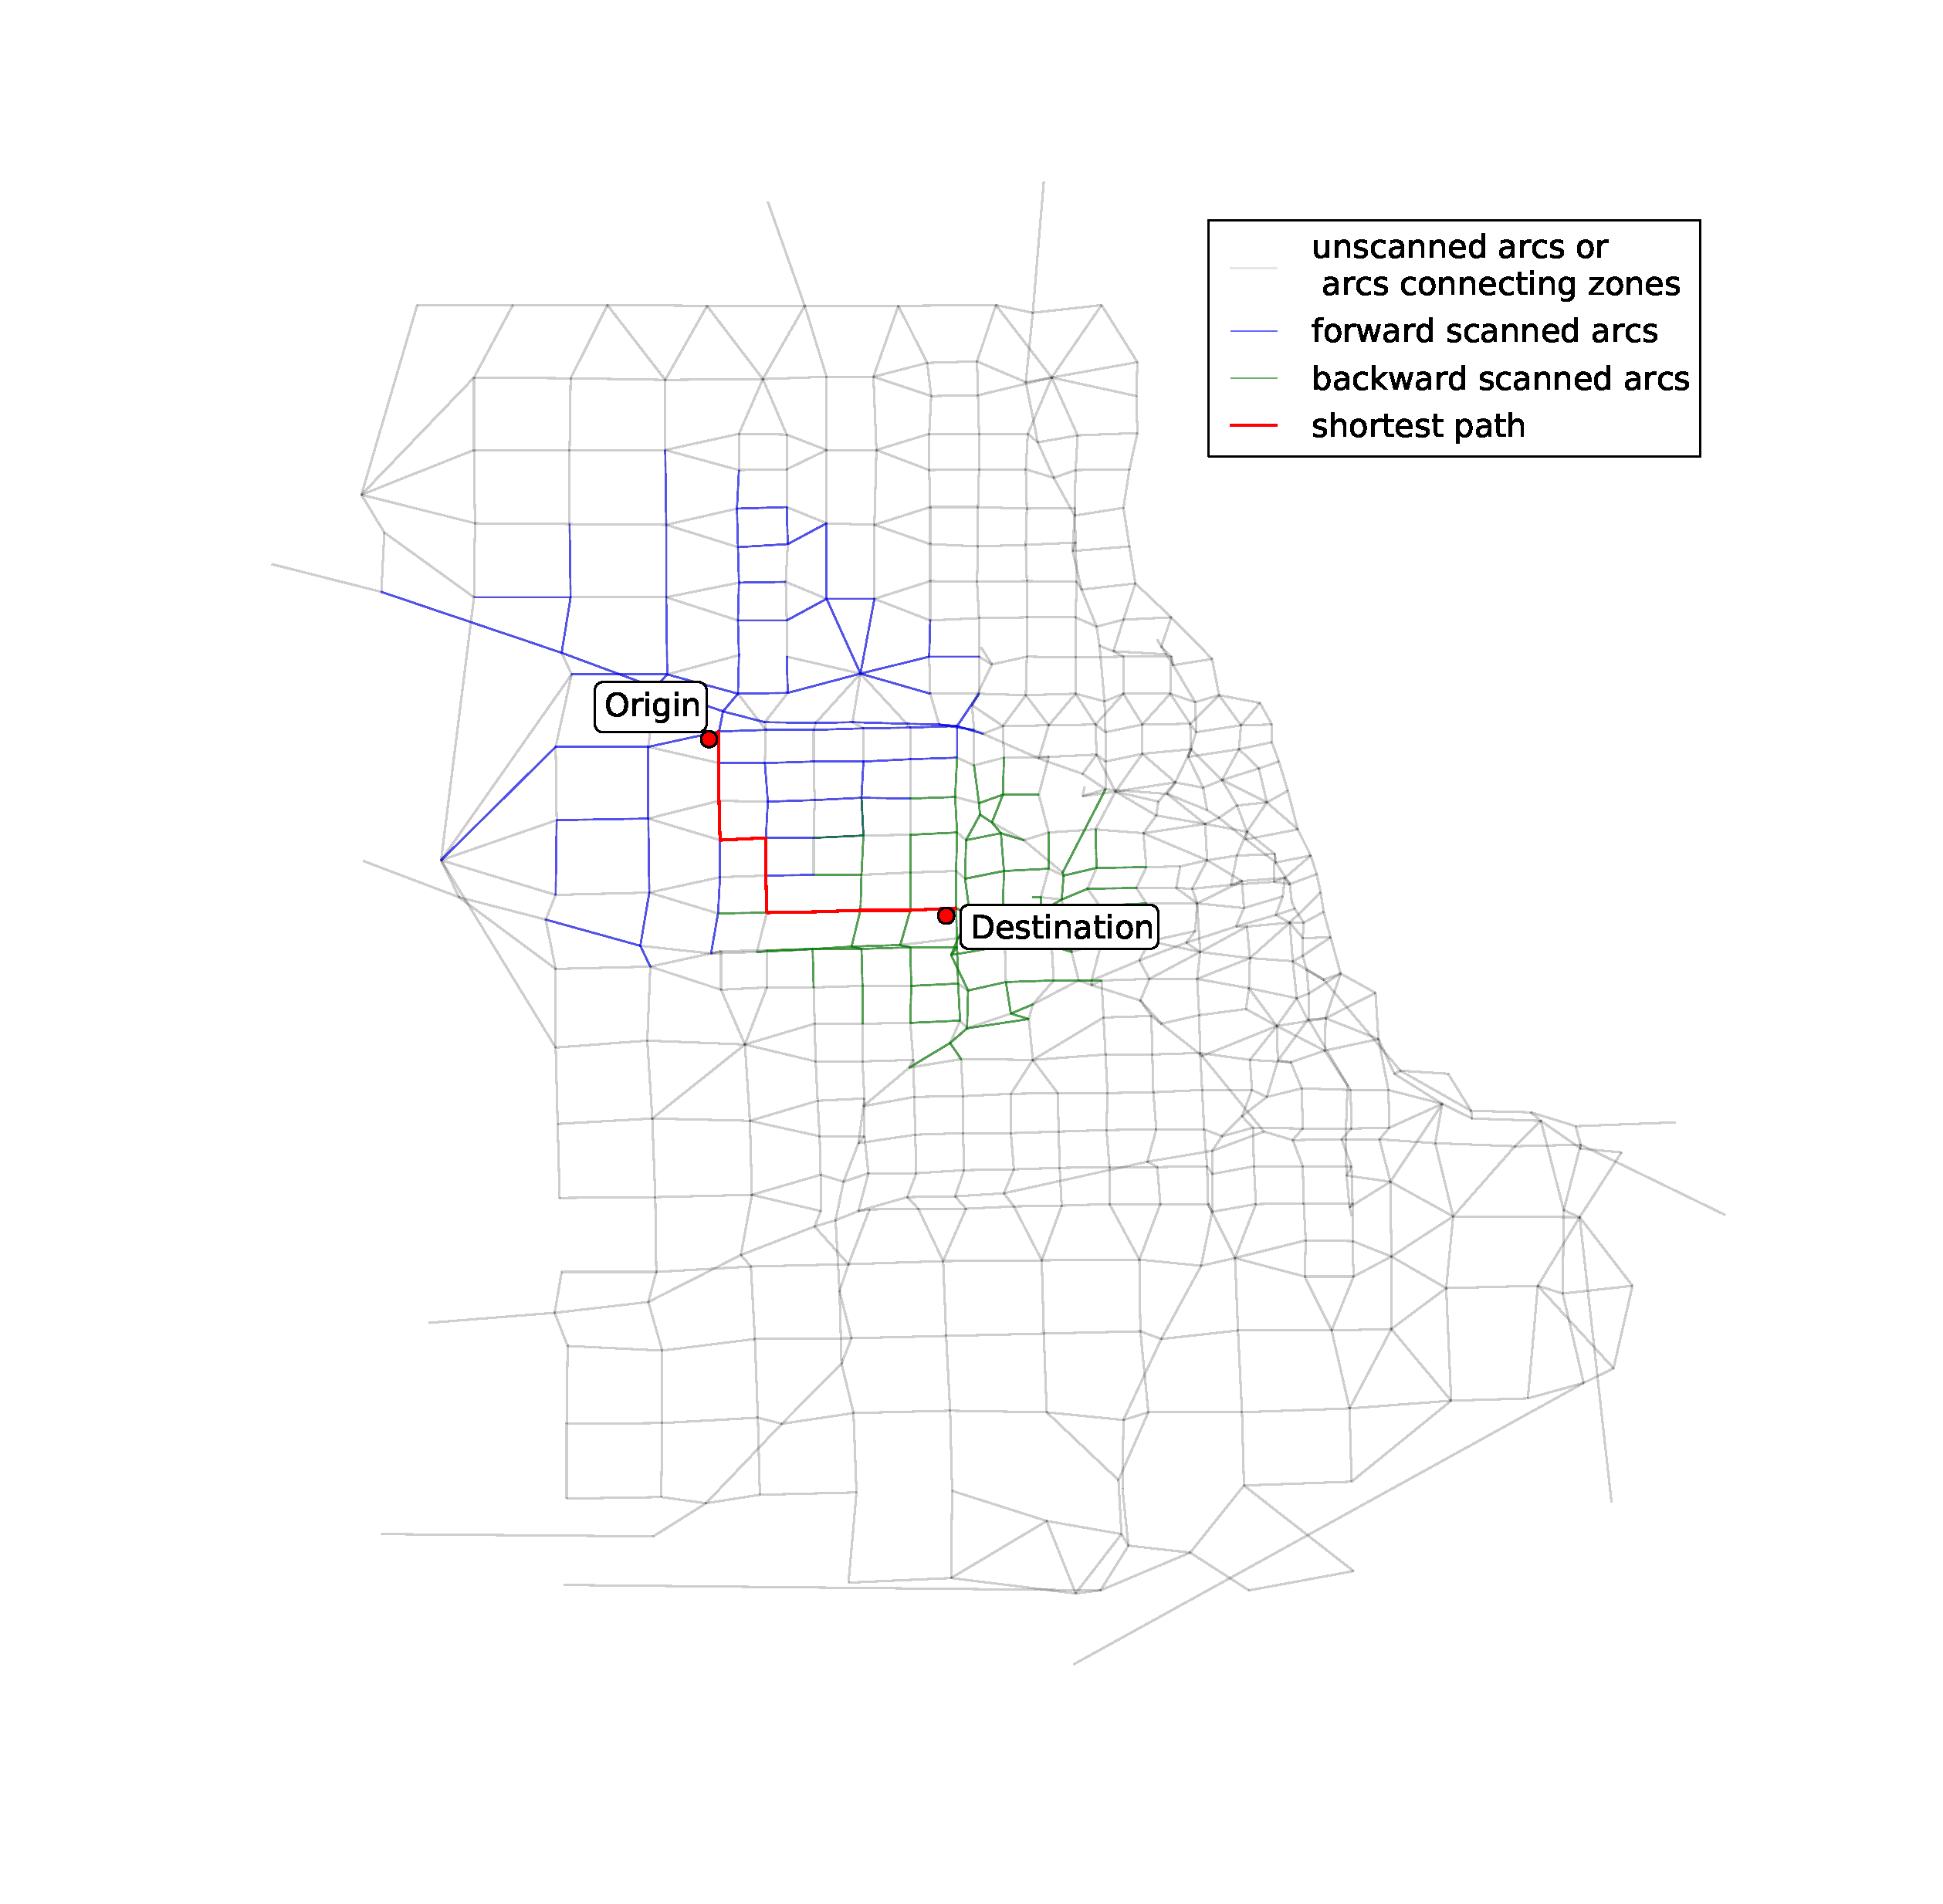
\includegraphics[width=\textwidth,trim=120px 120px 48px 120px,clip]{img/chicago_bidirect2}
        \caption{Bidirectional Dijkstra}
        \label{fig:chicago_bidirect2}
    \end{subfigure}
    \begin{subfigure}{.5\textwidth}
        \centering
        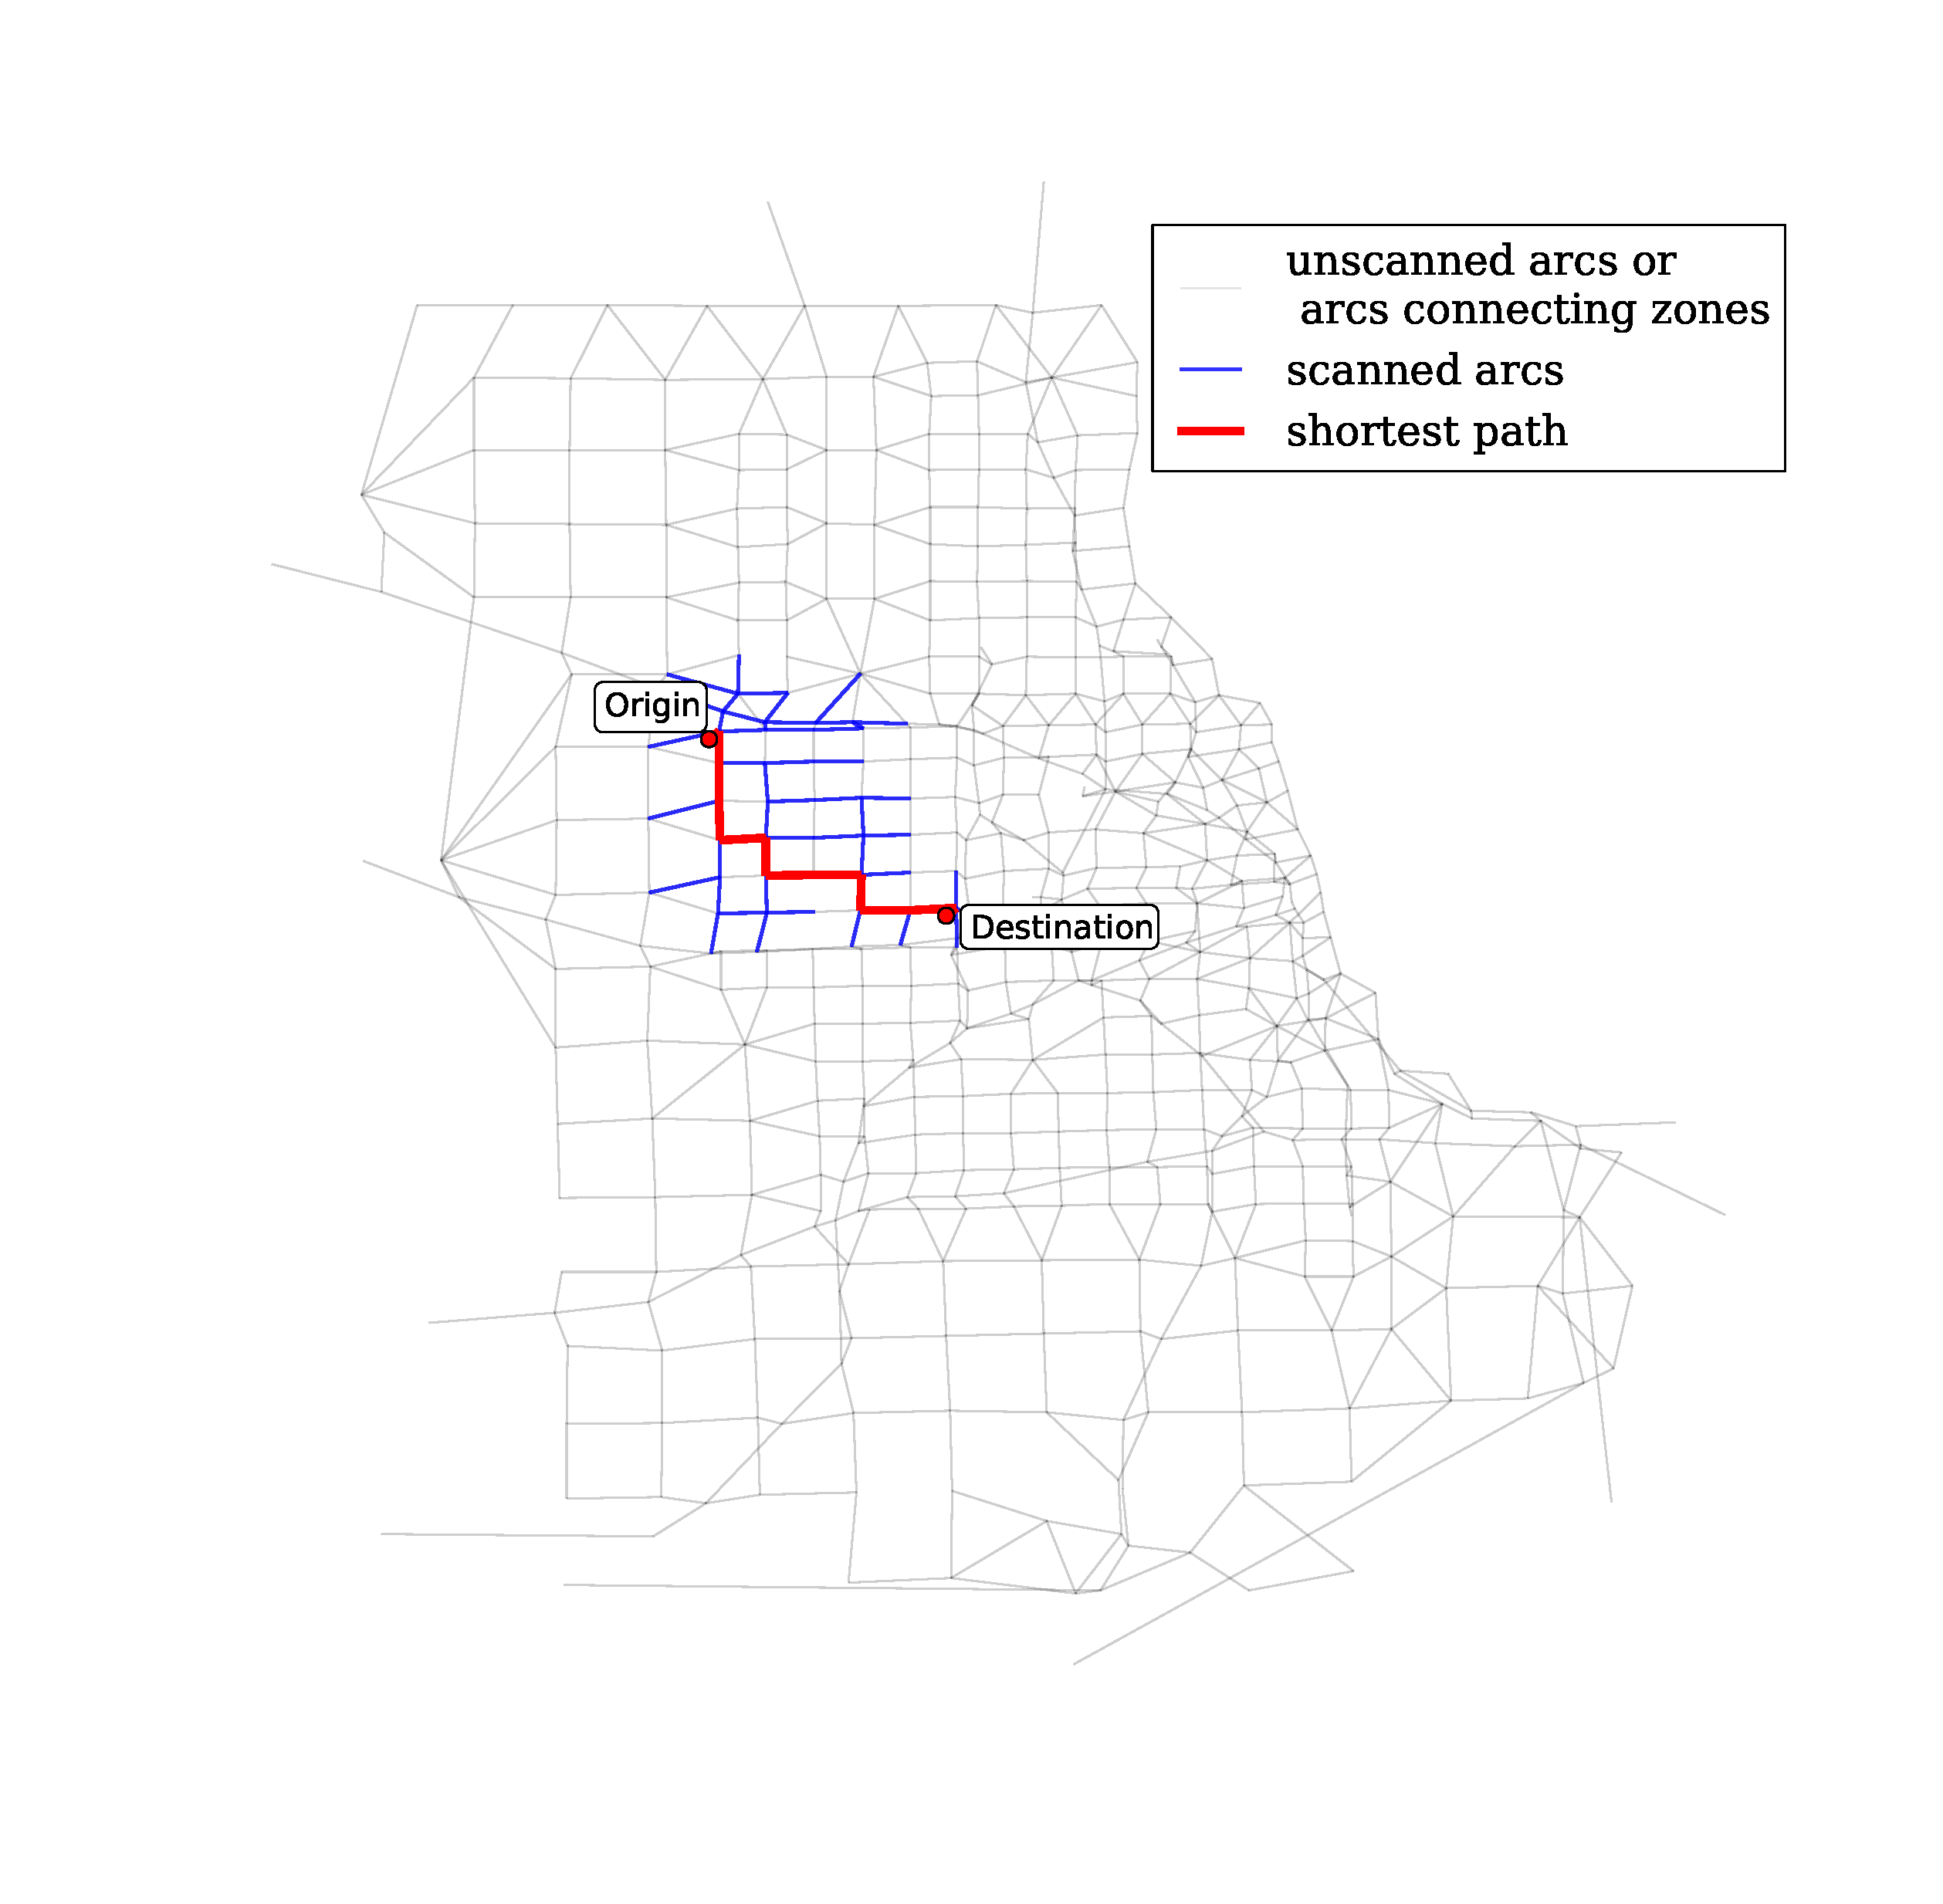
\includegraphics[width=\textwidth,trim=120px 120px 48px 0px,clip]{img/chicago_astar2}
        \caption{A* Search}
        \label{fig:chicago_astar2}
    \end{subfigure}%
    \begin{subfigure}{.5\textwidth}
        \centering
        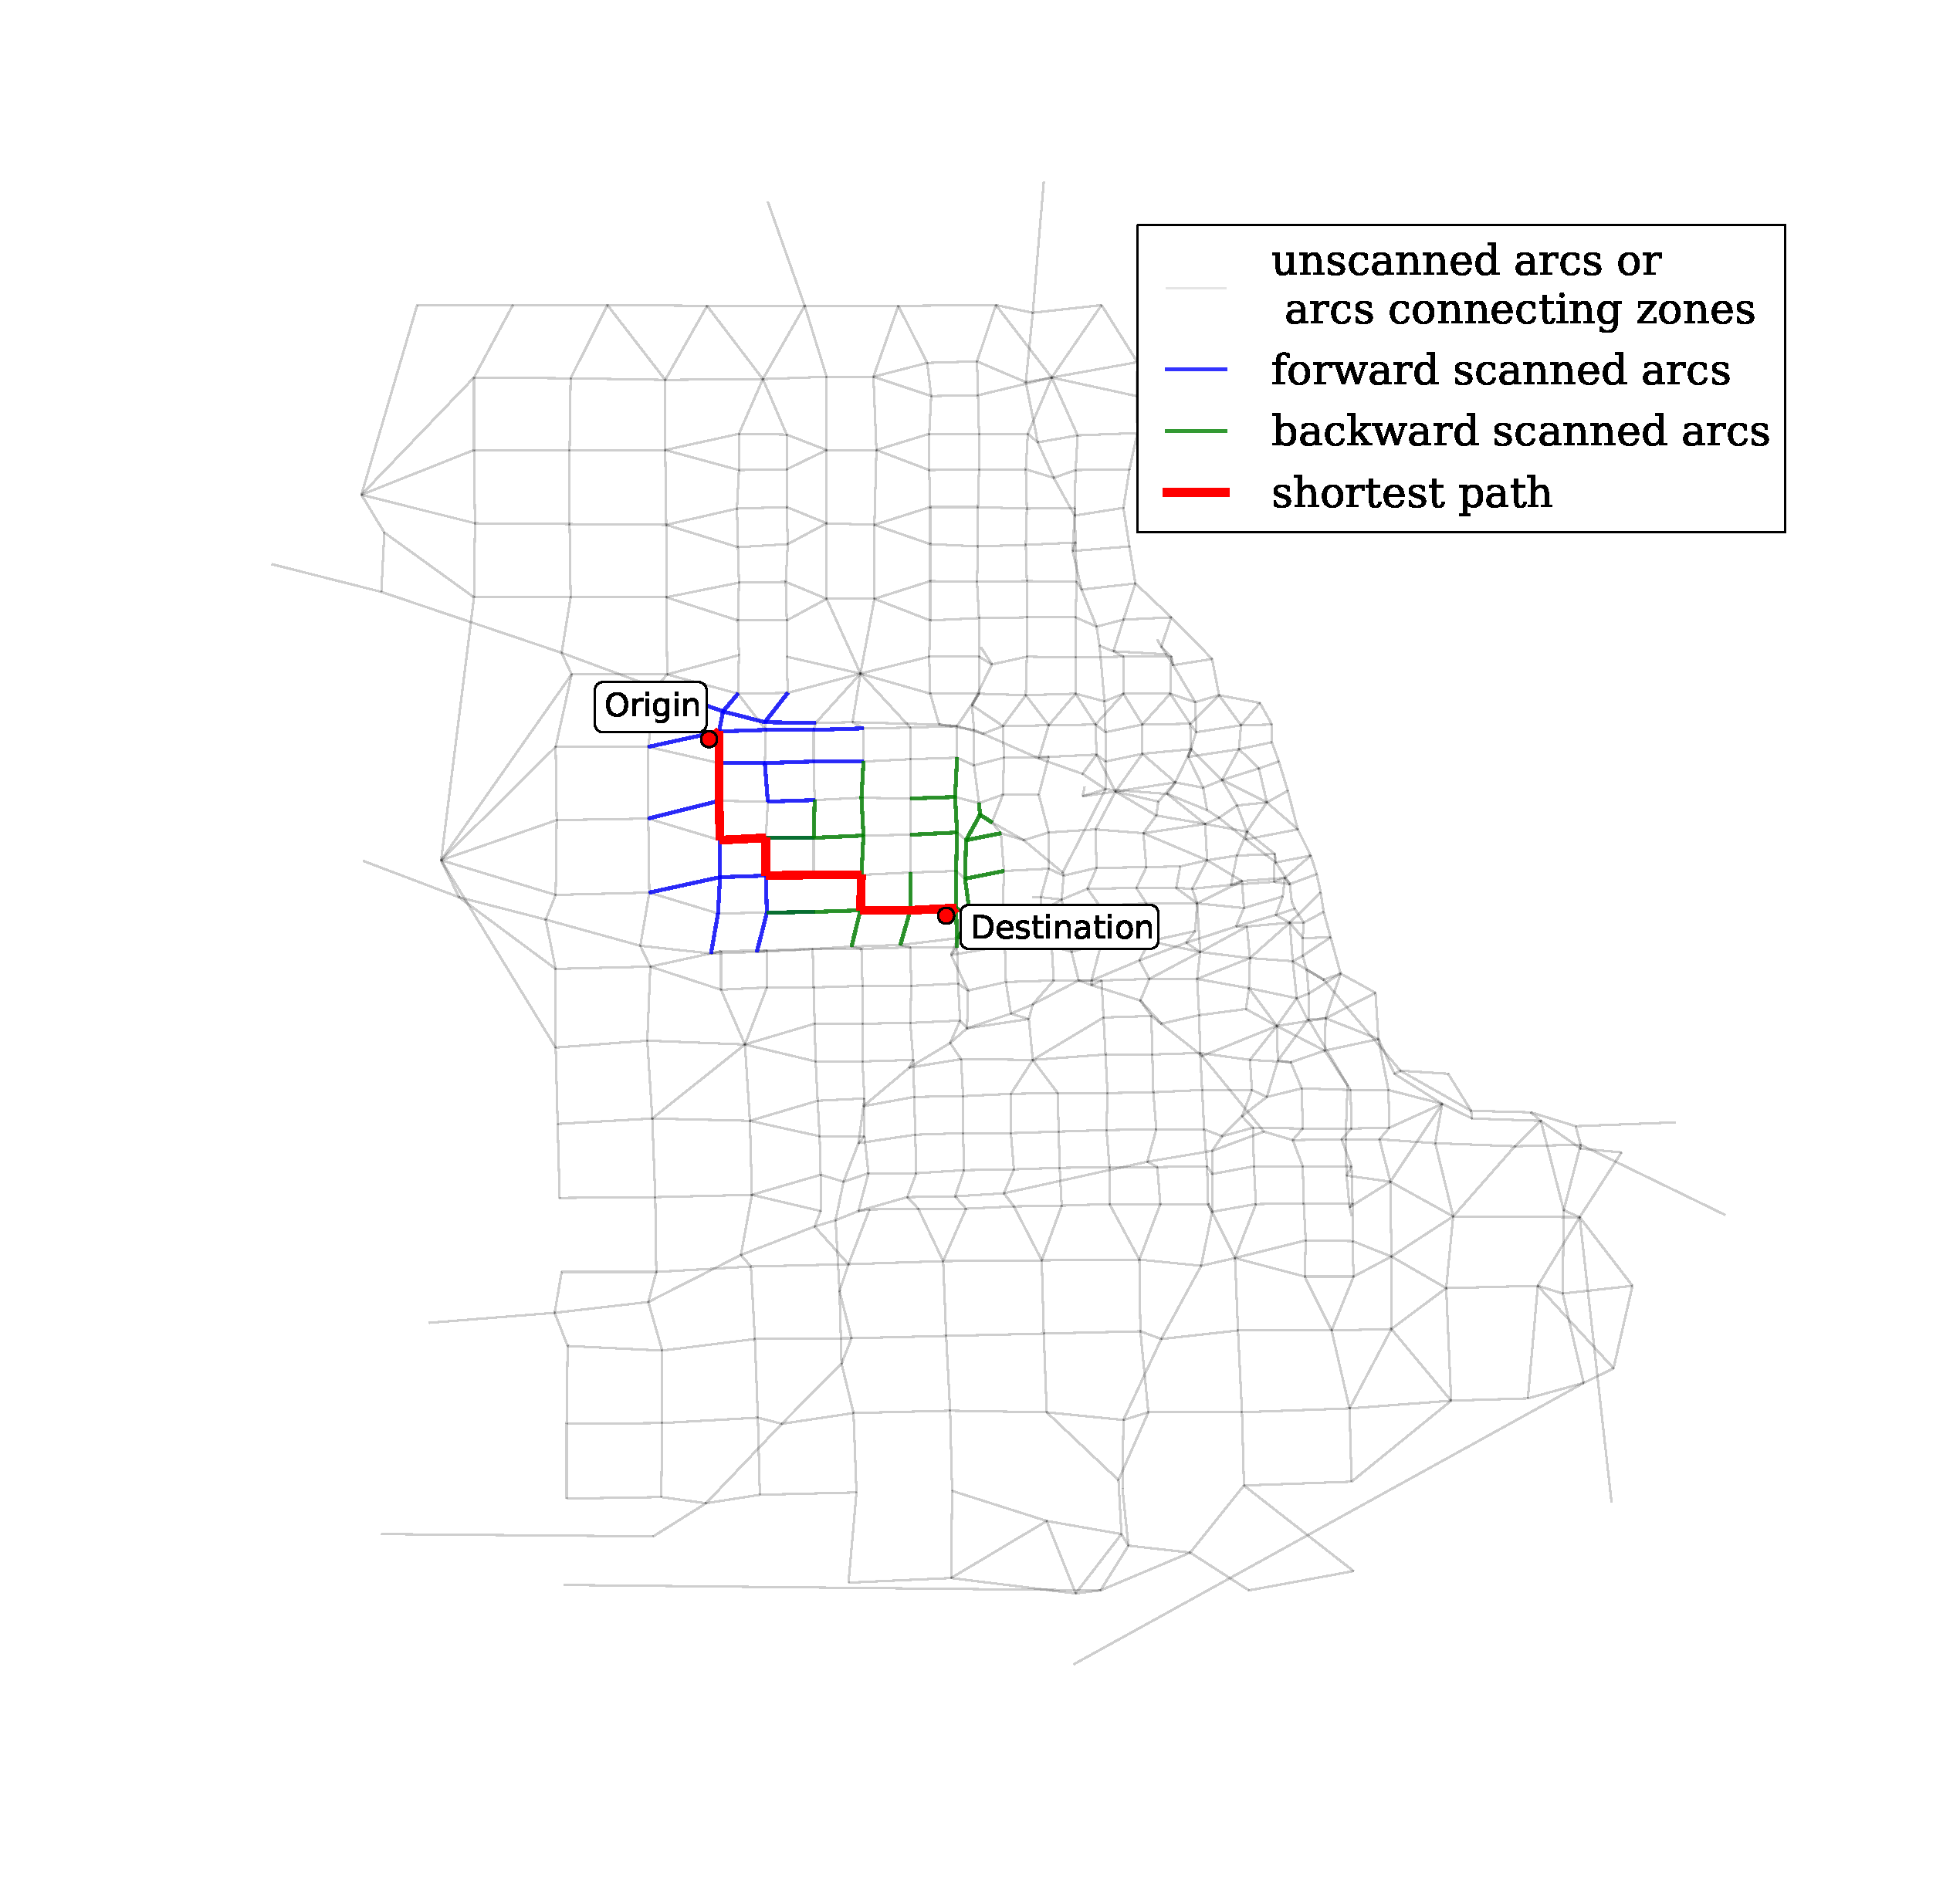
\includegraphics[width=\textwidth,trim=120px 120px 48px 0px,clip]{img/chicago_astar_bidirect2}
        \caption{Bidirectional A* Search}
        \label{fig:chicago_astar_bidirect2}
    \end{subfigure}
    \vspace{1em}
    \caption{Shortest path tree between two close nodes in the ChicagoSketch Network}
    \label{fig:short_sptree}
\end{figure}

\section{A* search with landmarks}
A* search with landmarks algorithm is not implemented for this project.
This is due to two reasons.
The first reason is due to its sophisticated graph dependent implementation,
where we need to either manually or dynamically decide the number of landmarks and their placement locations.
The second reason is due to its high chance of not being able to work,
as the algorithm is aimed at geographic node locations and Euclidean distances,
not our travel times that based on traffic flows.

Preprocessing algorithms are not really practical for the traffic assignment problem and the transportation forecasting model.
This is because normally these algorithms tend to spend much longer time than just running its standard version.
And since the purpose of the traffic assignment is to modify the network and resolve the problem to see its affect on congestion,
so it is not ideal to rerun the preprocessing algorithm every time the network is modified.


\newpage
\chapter{Summary and conclusions} \label{chap:conclusions}
To summarise,
in this project we have studied the point-to-point shortest path problem embedded in the path equilibration algorithm for solving the traffic assignment problem.
We have implemented Dijkstra's algorithm, A* search and their bidirectional versions.
Two strategies were developed to improve the performance of these shortest path algorithms when they are used in the iterative path equilibration algorithm.
The first strategy is to avoid the next few number of iterations
when the shortest path of the previous two iterations are the same.
The second strategy is to randomly skip the next shortest path calculation,
where we hope for the shortest path in the current and previous iteration is going to be the same.
In addition,
we have also investigated the possibility of using preprocessing methods such as A* search with landmarks algorithm.

We now conclude this project with the following points:
\begin{itemize}
    \item The A* search algorithm using zero-flow travel times as heuristic estimates has the best performance.
    \item Bidirectional versions of Dijkstra's algorithm and the A* search have worse performances. Bidirectional Dijkstra is worse because its need to check the stopping criterion at each step. Bidirectional A* is worse because its search area is larger than unidirectional A*.
    \item The strategy of avoiding next few iterations of shortest path calculations is not viable as it is difficult to find the best number of iterations to skip.
    \item The strategy of avoiding shortest path calculations randomly is viable. By using A* search and 50\% random skipping on large networks that require millions of shortest path calculations in each iteration, the run times are further improved by about 25\% compared to just using A* search.
    %\item Preprocessing shortest path algorithms are not applicable for the traffic assignment problem, due to their long preprocessing time can slow down the whole traffic assignment process when the road network need to be changed frequently.
    \item A* search with landmarks is not applicable unless we decide to concentrate on a specific road network, for example the Auckland Regional Transport model.
\end{itemize}

\section{Future work}
The current A* search algorithm only runs on a single thread.
The algorithm can be improved by implementing a multi-threaded version developed
by \citet{Inam}.
The algorithm will run extremely fast as it is designed for GPGPU (General Purpose GPU) run on multi processors using many threads concurrently.
The main modification of the algorithm is that  
instead of sequentially update all emanating arcs from the labelled node,
we update them in parallel using multiple threads.

A* search with landmarks algorithm can be investigated
if we decide to concentrate on a specific road network.
How many landmarks need to be used and where to place them need to be experimented in order to find the best combination of preprocessing run time and actual query time.


\newpage
%\appendix
%\begin{appendices}
%\end{appendices}


\newpage
\bibliographystyle{agsm}
\renewcommand{\bibname}{References}
\bibliography{citations}

\end{document}
